% !TEX program = xelatex
\documentclass[12pt,a4paper,openany]{ctexrep}

\usepackage{geometry}
\geometry{margin=2.5cm}
\usepackage{amsmath,amssymb,bm,mathtools}
\usepackage{graphicx}
\usepackage{booktabs}
\usepackage{multirow}
\usepackage{array}
\usepackage{longtable}
\usepackage{hyperref}
\usepackage{xcolor}
\usepackage{setspace}
\usepackage{caption}
\usepackage{subcaption}
\usepackage{algorithm}
\usepackage{algpseudocode}
\usepackage{enumitem}
\usepackage{float}
\usepackage{cite}

\onehalfspacing
\hypersetup{colorlinks=true,linkcolor=black,citecolor=blue,urlcolor=blue}
\captionsetup{font=small,labelfont=bf}
\graphicspath{{figures/}}

\title{\textbf{基于再生核希尔伯特空间的\\大规模 MU-MIMO 符号检测研究报告}}
\author{课题组\quad RKHS 优化问题}
\date{\today}

\begin{document}
\maketitle
\begin{abstract}
\noindent
大规模多用户多输入多输出（MU-MIMO）系统中，基站需在多用户干扰与有限信道状态信息（CSI）条件下完成可靠符号检测。最大似然检测（MLD）在贝叶斯意义下最优，但其复杂度随用户数指数增长；线性最小均方误差（MMSE）检测可部署，但在低中信噪比与强干扰场景性能受限。深度学习检测器近年取得进展，却往往依赖大量标注、可解释性不足，且对 CSI 误差敏感。

本报告研究一类以\textbf{再生核希尔伯特空间（RKHS）}为假设类、以\textbf{贝叶斯后验损失}为目标的检测框架。决策始终保持
\[
L(y)=K_\eta(\varphi(y),C)\alpha^\top,\qquad \hat X_1=\arg\max_a L_a(y)
\]
的核展开形式。针对可部署约束（无真信道 $H$、无真后验 $f^*$ 监督），提出稳健结构化特征 $z_{\mathrm{rob}}(y;\hat H)$，并在 Adaptive-MKL、核内神经网络系数生成、验证集聚合与可选二阶堆叠等模块上强化表达能力。同时，以真 $H$ 的 struct 特征拟合 $f^*$ 构造 RKHS Oracle，实证说明：在合适核空间中可任意逼近贝叶斯后验。

在 $M=128$、$K=40$、16/64-QAM、仅检测期望用户 $X_1$ 的设定下，实验表明：可部署 RKHS 相对 MMSE+LS 在 16-QAM、0--10\,dB 降低误比特率约 19\%--35\%；在多种前端失真下相对增益可进一步扩大；Oracle 与 MLD 高度一致。报告系统阐述问题背景、研究现状、理论基础、方法细节、实现要点与实验结果，并讨论局限与后续方向。
\end{abstract}

\tableofcontents
\clearpage

\chapter{绪论：问题背景与研究动机}

\section{从多用户接入到符号检测}

无线通信的核心任务之一，是在噪声与干扰下从接收波形中恢复发射端所传的数字符号。对单用户加性高斯白噪声（AWGN）信道，匹配滤波加硬判决在充分统计意义下已是最优；一旦多个用户在同一时频资源上叠加——无论是码分多址、OFDMA 上行还是空间复用 MIMO——接收机面对的就是经典的\textbf{多用户检测（multiuser detection）}问题\cite{verdú1998,tse2005}：需要在多址干扰（MAI）与噪声并存时，推断一个或多个用户的符号。

进入 4G/5G 时代，基站侧大规模天线阵列使频谱效率显著提升\cite{marzetta2010,larsson2014,bjornson2017}。上行多用户 MIMO（MU-MIMO）中，$K$ 个用户同时向配备 $M$ 根天线的基站发射，基带等价模型通常写为
\begin{equation}
\mathbf{y}=\mathbf{H}\mathbf{x}+\mathbf{n},
\label{eq:mimo-basic}
\end{equation}
其中 $\mathbf{y}\in\mathbb{C}^{M}$ 为接收向量，$\mathbf{H}\in\mathbb{C}^{M\times K}$ 为信道矩阵，$\mathbf{x}=(x_1,\ldots,x_K)^\top$ 各分量取自有限星座 $\mathcal{A}$（如 QPSK、16-QAM），$\mathbf{n}$ 为圆对称复高斯噪声。\textbf{符号检测}即：在已知或估计得到的 $\mathbf{H}$ 下，由 $\mathbf{y}$ 给出 $\mathbf{x}$ 的硬判决或软信息（LLR），供后续译码使用。

检测问题的难度由三方面共同决定：
\begin{enumerate}[leftmargin=2em]
  \item \textbf{维数}：$K$ 增大使联合假设空间 $|\mathcal{A}|^K$ 指数膨胀；
  \item \textbf{几何}：$\mathbf{H}$ 的条件数、用户相关性决定干扰可分程度；
  \item \textbf{信息}：信道状态信息（CSI）是否完美、噪声与干扰统计是否准确。
\end{enumerate}
当 $M\gg K$ 且信道近似正交时，简单线性接收机已接近最优\cite{hoydis2013}；但当 $K/M$ 不可忽略、SNR 处于低中区间、或 CSI 存在误差时，线性方法与最优检测之间仍存在可观间隙——这也是本报告关注 $M=128$、$K=40$、0--10\,dB 设定的原因。

\section{信号检测的基本模型分层}

为便于后文对照，将常见检测模型按“观测--假设--准则”分层简述。

\subsection{假设检验视角}
给定 $\mathbf{H}$（或其后验），检测是离散参数的假设检验：每个候选 $\mathbf{x}\in\mathcal{A}^K$ 对应一个均值 $\mathbf{H}\mathbf{x}$。最大似然（ML）准则为
\begin{equation}
\hat{\mathbf{x}}_{\mathrm{ML}}
=\arg\min_{\mathbf{x}\in\mathcal{A}^K}\|\mathbf{y}-\mathbf{H}\mathbf{x}\|^2.
\label{eq:ml}
\end{equation}
在均匀先验下 ML 与最大后验（MAP）一致。若只关心某一用户 $x_1$，则最优是对联合后验做\textbf{边际化}：
\begin{equation}
\hat x_1^{\mathrm{MAP}}
=\arg\max_{a\in\mathcal{A}}
\sum_{\mathbf{x}_{2:K}\in\mathcal{A}^{K-1}}
\mathbb{P}(\mathbf{x}=(a,\mathbf{x}_{2:K})\mid\mathbf{y}),
\end{equation}
其计算同样涉及指数级求和，是“只检单用户”时的贝叶斯金标准。

\subsection{线性模型族}
将 $\mathbf{x}$ 暂视为连续变量，可得到闭式线性估计再量化到星座：
\begin{itemize}
  \item \textbf{匹配滤波（MF）}：$\hat{\mathbf{x}}\propto \mathbf{H}^H\mathbf{y}$，忽略用户间干扰；
  \item \textbf{迫零（ZF）}：$\hat{\mathbf{x}}=(\mathbf{H}^H\mathbf{H})^{-1}\mathbf{H}^H\mathbf{y}$，消除干扰但放大噪声；
  \item \textbf{线性 MMSE}：
  \begin{equation}
  \hat{\mathbf{x}}_{\mathrm{MMSE}}
  =\mathbf{H}^H\big(\mathbf{H}\mathbf{H}^H+N_0\mathbf{I}\big)^{-1}\mathbf{y},
  \end{equation}
  在均方误差意义下最优的线性估计，并可理解为对干扰加噪声的折中加载\cite{kay1993,tse2005}。
\end{itemize}
工程上常配合导频得到 $\hat{\mathbf{H}}$，即本报告基线 \textbf{MMSE+LS}。线性族复杂度约为矩阵求逆量级，可实时部署，但在强干扰/低 SNR 下 BER 距 ML 较远。

\subsection{非线性与搜索类模型}
\begin{itemize}
  \item \textbf{串行/并行干扰消除（SIC/PIC）}：用已检符号重构干扰并相减，可与排序、软估计结合；
  \item \textbf{球形译码（Sphere Decoding）}：在半径约束内搜索靠近 $\mathbf{y}$ 的格点，逼近 ML，但高维时节点访问量仍可能指数增长\cite{hassibi2005,studer2011}，大规模配置下常被视为难以直接部署\cite{larsson2014}；
  \item \textbf{格基约减 + 线性均衡}：改善信道基底后再做 ZF/MMSE，属于性能--复杂度折中。
\end{itemize}
此外，近似消息传递（AMP/OAMP 等）在大系统极限下有严密分析，并常被深度学习展开\cite{he2018}。这类方法依赖信道与先验结构假设，本项目未以其为主线，但后文稳健充分统计中的高斯干扰近似与之精神相近。

\subsection{学习型检测模型}
近年来，深度网络被用于直接学习 $\mathbf{y}\mapsto\mathbf{x}$ 或算法展开\cite{samuel2019,o2017,khani2020}。其模型可概括为：用参数函数 $f_\theta$ 近似 MAP/迭代接收机映射，用交叉熵或均方损失在仿真数据上训练。优点是表达力强；挑战是可解释性、CSI 失配下的稳健性，以及与通信最优准则的对齐程度。本报告以 CNN 作为该类基线之一，而主方法采用\textbf{保留核决策形式}的 RKHS 学习，以便与贝叶斯后验损失严格对应。

\section{问题背景：性能、复杂度与 CSI 三重张力}

综合上述模型，当代上行 MU-MIMO 检测处在三重张力之中：

\paragraph{（1）最优性 vs 复杂度}
ML/MAP 与精确边际化在星座离散约束下最优，但复杂度随 $K$ 与调制阶数指数上升；球形译码等可降低平均复杂度，却难以保证最坏情况实时性。因此，可部署接收机长期以线性 MMSE 及其迭代变形为主。

\paragraph{（2）天线数优势 vs 负荷比}
大规模 MIMO 的“信道硬化、渐近正交”论证的是 $M/K\to\infty$ 时线性接收足够好\cite{marzetta2010,hoydis2013}。当 $K$ 与 $M$ 同量级（本报告 $40/128$）或工作在低中 SNR 时，线性方法留有改进空间——文献亦指出天线--用户比较低时经典检测性能明显恶化，从而激发学习检测等研究\cite{khani2020}。

\paragraph{（3）完美 CSI 假设 vs 可部署估计}
多数检测推导默认 $\mathbf{H}$ 已知。实际中 $\mathbf{H}$ 由上行导频估计，存在噪声、污染与校准误差\cite{bjornson2017}。把 $\hat{\mathbf{H}}$ 直接代入 ML/MMSE 公式，等价于错误指定模型：高 SNR 下估计误差会被放大，表现为“越信噪比越高越脆弱”。因此，任何宣称可上线的学习检测，都必须明确训练/测试期可用的信息集。

本报告正是在这三重张力下选题：\textbf{不追求联合 ML 搜索}，而追求在可部署信息集上，用有理论结构的函数类逼近单用户贝叶斯最优，并尽量超过 MMSE+LS。

\section{本项目的问题设定（方案 A）}

我们采用\textbf{方案 A}：不联合恢复全部 $K$ 个符号，只检测期望用户 $x_1\in\mathcal{A}$，其余用户 $\mathbf{x}_I=(x_2,\ldots,x_K)$ 视为干扰。该设定的背景含义是：
\begin{enumerate}[leftmargin=2em]
  \item \textbf{业务不对称}：调度用户、测量用户或某一逻辑流的数据才是当前关心对象；
  \item \textbf{复杂度接口}：把 $|\mathcal{A}|^K$ 联合问题降为“干扰环境下的 $|\mathcal{A}|$ 元检测”，使核方法/学习方法输入规模可控；
  \item \textbf{最优准则清晰}：贝叶斯最优由后验
  \[
  f_a^*(\mathbf{y})=\mathbb{P}(x_1=a\mid\mathbf{y})
  \]
  的最大元给出；学习目标可直接取后验交叉熵型损失，而不是间接模仿某一线性接收机残差。
\end{enumerate}
精确 $f_a^*$ 需对 $\mathbf{x}_I$ 边际化；实践中可用蒙特卡洛或\textbf{高斯干扰近似（GA）}得到软分，后者并构成本方法结构化特征的物理来源。

仿真默认：$M=128$，$K=40$，方形 QAM（主结果 16-QAM，扩展含 64-QAM），$Y=H_{\mathrm{eff}}X+N$ 的块衰落 Rayleigh 等效信道；指标为 Gray 标注下期望用户的 bit BER。

\section{可部署约束与 Oracle 的分工}

\textbf{可部署主线}要求：
\begin{enumerate}[leftmargin=2em]
  \item 测试期不使用真 $H$，只使用导频 LS 的 $\hat H$ 与 $\hat N_0$；
  \item 不使用真后验 $f^*$ 作监督（可用仿真得到的真实符号 $x_1$ 作硬标签，对应离线有监督训练）；
  \item 主目标是降低相对 MMSE+LS 的 BER，而非仅拟合某一中间统计量。
\end{enumerate}
\textbf{RKHS Oracle}则故意使用真 $H$ 与真 $f^*$，用于检验：在合适特征坐标上，再生核希尔伯特空间是否足以逼近贝叶斯后验（逼近 MLD）。二者决策形式相同，信息集不同，避免把“上界实验”与“上线方案”混为一谈。

\section{方法路线预告：为何是 RKHS}

在明确检测模型与信息约束后，本工作选择 RKHS 作为假设类\cite{aronszajn1950,schafer2006,steinwart2008}：表示定理保证解为有限核展开；通用核提供逼近能力；正则项 $\|f\|_{\mathcal{H}}^2$ 与泛化分析清楚。关键并非“用核直接分类原始 $\mathbf{y}$”，而是先构造与 GA-MLD 对齐的充分统计特征（可部署时为稳健的 $z_{\mathrm{rob}}(\hat H)$），再在该空间上最小化贝叶斯后验损失
\begin{equation}
J(f)=\mathbb{E}\Big[-\log\frac{f_{x_1}(Y)}{\sum_b f_b(Y)}\Big]+\lambda\|f\|_{\mathcal{H}}^2.
\end{equation}
这一“\textbf{通信模型启发的特征 + 核空间中的贝叶斯风险最小化}”构成后续章节的主线。

\section{研究目标与报告结构}

\noindent\textbf{目标：}在 $128\times40$、16-QAM、只检 $x_1$ 设定下，得到可部署 RKHS 检测器，使其 BER 显著优于 MMSE+LS；并用 Oracle 验证 struct 坐标上 RKHS 对 $f^*$ 的可逼近性。

\noindent\textbf{结构：}第\ref{ch:survey}章综述；第\ref{ch:model}章系统模型；第\ref{ch:theory}章方法要点；第\ref{ch:method}--\ref{ch:impl}章方法与实现；第\ref{ch:exp}章实验与结果；第\ref{ch:discuss}章结论。学术证明另册，不纳入本交付正文。

\chapter{研究现状与相关工作}
\label{ch:survey}

本章沿“经典统计检测 $\to$ 大规模 MIMO 实用接收 $\to$ 迭代/消息传递 $\to$ 深度学习检测 $\to$ 核方法与稳健 CSI $\to$ 研究空白”的脉络梳理现状，并明确本工作的定位。

\section{经典多用户检测理论}

多用户检测的系统框架由 Verdú 等奠定\cite{verdú1998}：在高斯多址模型下，最优多用户检测、匹配滤波、解相关器与线性 MMSE 接收机构成清晰的性能--复杂度谱系。其核心洞见是：匹配滤波在多用户场景一般\textbf{不是}单用户最优的简单推广；利用干扰结构可显著降低误码。

对空间复用 MIMO，联合最大似然（ML）检测等价于有限星座上的最小距离搜索。球形译码（SD）及其软输入软输出变体通过树搜索逼近 ML，并可为信道译码器提供 LLR\cite{hassibi2005,hochwald2003,studer2011}。K-best、固定复杂度球译码等变体以可预测时延换取次优。然而当用户数 $K$ 与调制阶数同时增大（如 $K=40$、16-QAM），联合搜索即便经过剪枝，最坏情况复杂度仍难以满足基站实时处理约束；因而工业界上行接收长期以线性或轻度非线性算法为主。

\section{大规模 MIMO 下的线性与正则化接收}

大规模 MIMO 改变了检测问题的“典型工作点”\cite{marzetta2010,larsson2014,bjornson2017}：当 $M\gg K$ 时，信道硬化与渐近正交使匹配滤波/MF 与 MMSE 的性能迅速靠近最优\cite{hoydis2013}。实用算法谱系包括：
\begin{itemize}
  \item \textbf{MF / ZF / MMSE}：闭式线性估计加硬判决；MMSE 在干扰抑制与噪声放大之间折中，并可视为对角加载\cite{tse2005,kay1993}；
  \item \textbf{正则化 ZF 与加载因子选择}：用渐近确定性等价或仿真标定正则参数；
  \item \textbf{迭代求逆近似}：Neumann 级数、Gauss--Seidel、共轭梯度等，降低大规模矩阵求逆成本。
\end{itemize}
\textbf{MMSE+导频估计}因此成为可部署基线的“强标准答案”。本报告以其为主要对照，而非设立一个容易击败的弱基线。

需要强调的现状是：文献中“线性已足够”的结论高度依赖 $M/K$ 很大、SNR 不太低、CSI 质量较高等条件。当负荷比升高（本报告 $K/M=40/128$）或工作在 0--10\,dB 低中 SNR 时，线性接收与 MAP/ML 之间仍常存在可观 BER 间隙——这也是学习检测与非线性检测持续被研究的原因。

\section{干扰消除、格方法与近似消息传递}

在线性接收之上，研究界发展了多类增强：
\begin{enumerate}[leftmargin=2em]
  \item \textbf{SIC/PIC}：用硬/软符号重构干扰并消除；排序、可靠度加权影响误差传播；
  \item \textbf{格基约减 + 均衡}：改善等效信道条件数后再做 ZF/MMSE；
  \item \textbf{EP / AMP / GAMP / OAMP}：在大系统极限下具有状态演化分析，能逼近贝叶斯最优的某类可计算近似，并对相关信道有扩展（如 OAMP）\cite{he2018}。
\end{enumerate}
这些方法在\textbf{完美或高质量 CSI}下表现突出。它们与本工作的联系在于：高斯干扰近似、协方差白化等思想会出现在充分统计构造中；差异在于本项目最终决策落在 RKHS 假设类上最小化后验损失，而不是把 PIC/AMP 迭代本身作为主检测器。项目早期曾试验 residual/PIC 前端，实验上未成为优于 $z_{\mathrm{rob}}$+RKHS 的默认可部署路径。

\section{深度学习检测：数据驱动与模型展开}

物理层深度学习综述表明，上行大规模 MIMO 检测已成为 DL 应用的热点之一\cite{o2017}。按架构大致可分为两类\cite{samuel2019,he2018,khani2020}。

\subsection{数据驱动（黑盒）网络}
以 $\mathbf{y}$ 或 $(\mathbf{y},\hat{\mathbf{H}})$ 为输入，多层网络直接输出符号/比特软信息。优点是表达力强、可端到端训练；缺点是参数量大、可解释性弱、对信道分布偏移敏感，且多数工作默认较理想的 CSI。

\subsection{模型驱动展开（deep unfolding）}
将经典迭代检测的每一步展开为网络层，只学习少量参数。代表性工作包括：
\begin{itemize}
  \item \textbf{DetNet}：展开投影梯度型迭代，展示 DL 做 MIMO 检测的可行性\cite{samuel2019}；
  \item \textbf{OAMP-Net / OAMP-Net2}：展开正交近似消息传递，参数更少，并讨论与信道估计结合的不完美 CSI 情形\cite{he2018}；
  \item \textbf{MMNet 等}：面向相关信道的展开检测，强调经典线性方法在相关信道上的不足\cite{khani2020}。
\end{itemize}
现状共识可概括为：（i）展开往往比纯黑盒更稳、更省参；（ii）\textbf{底层迭代算法的选择常常比“多加几个可学习标量”更关键}；（iii）许多工作仍在相对较小的 $M,K$ 或较强 CSI 假设下评估；（iv）不完美 CSI、导频开销与跨 SNR 泛化仍是开放问题。

本报告用 CNN 作为深度学习对照，而不是复现全部 DetNet/OAMP-Net 族：目的是提供“数据驱动分类器”参照，主贡献放在\textbf{贝叶斯损失 + 结构化特征 + RKHS 决策形式}这一不同于展开网络的路线。

\section{核方法、多核学习及其在通信中的位置}

核方法通过再生核将线性算法隐式提升到高维特征空间\cite{schafer2006,shawe2004,vapnik1998}。高斯核等通用核在适当条件下具有万能逼近性质\cite{steinwart2008}；多核学习（MKL）在基核凸组合上学习权重，减轻核选择困难\cite{bach2004,micchelli2005,cortes2009,rakotomamonjy2008}。

在通信与信号处理中，核自适应滤波、高斯过程、核贝叶斯多用于信道预测、非线性均衡与调制识别等。直接把核分类器用在大规模 MU-MIMO 符号检测的系统工作相对少于深度学习。现有思路的常见不足是：
\begin{itemize}
  \item 输入仍用原始高维 $\mathbf{y}$，使后验在高 SNR 下极尖锐，核带宽难选；
  \item 损失与贝叶斯检测准则对齐不清晰；
  \item 未系统区分“特权信息上界”与“可部署信息集”。
\end{itemize}
本工作针对这些不足：以 16 维 GA/稳健软分为坐标、以 $J(f)$ 为训练目标、以 Adaptive-MKL/核内系数学习增强表达，并显式分开 Oracle 与可部署主线。

\section{不完美 CSI 与稳健接收现状}

不完美 CSI 下的稳健接收是经典课题\cite{kay1993,bjornson2017}：对角加载、最坏情况设计、贝叶斯估计--检测联合、以及把误差协方差并入干扰模型等。TDD 大规模 MIMO 还有导频污染问题\cite{marzetta2010}。深度学习检测文献也开始讨论联合信道估计与检测（JCESD）及估计误差感知训练\cite{he2018}，但总体仍少于完美 CSI 设定下的结果。

本报告采取可实现的中间路线：不宣称解决导频污染，而用导频 LS 误差方差 $\sigma_e^2$ 对干扰协方差做对角加载，得到 $z_{\mathrm{rob}}$。这与“加长导频硬追完美 CSI”不同——后者把增益押在估计质量上；我们把增益押在\textbf{检测器对估计误差的容忍与后验损失优化}上。

\section{评价准则与实验惯例}

文献中常见指标包括 SER/BER、与 ML 的差距、互信息/软输出质量、复杂度（FLOPs、时延）、以及跨信道相关模型/跨 SNR 的泛化。深度学习工作还常报告训练样本需求与在线推理时间。本报告主报：
\begin{itemize}
  \item 期望用户 bit BER（相对 MMSE 的增益）；
  \item 后验损失 $J$；
  \item Oracle 相对 MLD 的 BER/$J$/MSE（表达力上界）。
\end{itemize}
复杂度的严格实时基准留作后续工作。

\section{研究空白与本工作定位}

综合现状，可见如下空白与张力：
\begin{enumerate}[leftmargin=2em]
  \item 在 $K/M$ 不可忽略、低中 SNR、仅可部署 CSI 时，相对 MMSE 的\textbf{稳定可复现增益}仍有需求；
  \item 深度展开很强，但与“\textbf{保留表示定理型决策形式、直接最小化贝叶斯后验损失}”的核路线之间，系统对比与协同仍不足；
  \item 上界实验（真 $H$、$f^*$）与上线方案（$\hat H$、hard）常被混用，导致“可逼近性”与“可部署性”论证不清。
\end{enumerate}

\noindent\textbf{本工作定位：}在方案 A（只检 $x_1$）下，给出一条结构化 RKHS 检测主线——可部署时用 $z_{\mathrm{rob}}(\hat H)$+hard 追击 MMSE；Oracle 时用 $z(H)$+$f^*$ 验证核空间可逼近后验。它介于经典线性接收与黑盒/展开深度检测之间，强调\textbf{模型启发特征、贝叶斯准则与可分析假设类}的统一。

\chapter{系统模型与最优检测}
\label{ch:model}

本章给出上行 MU-MIMO 的观测与检测模型，并专门澄清：\textbf{线性与非线性在本问题中都可能存在}——前者主要体现在观测方程与线性接收机，后者主要体现在星座约束下的最优判决以及各类非线性接收机。二者不是互相否定，而是不同层次、不同工作条件下的可选形态。

\section{观测方程：对连续符号是线性的}

窄带块衰落上行 MU-MIMO 中，基站天线数 $M=128$，并发流数 $K=40$。等效基带模型为
\begin{equation}
Y = H_{\mathrm{eff}} X + N \in \mathbb{C}^{M},
\label{eq:sys}
\end{equation}
其中 $H_{\mathrm{eff}}\in\mathbb{C}^{M\times K}$ 为 Rayleigh 等效信道（仿真中直接生成），$X=(X_1,\ldots,X_K)^\top$ 各分量取自归一化方形 $M$-QAM 星座 $\mathcal{A}$（默认 $|\mathcal{A}|=16$，扩展实验含 $|\mathcal{A}|=64$，$E_s=1$，Gray I/Q 映射），$N\sim\mathcal{CN}(0,N_0 I)$。信噪比 $\mathrm{SNR}_{\mathrm{dB}}=10\log_{10}(E_s/N_0)$。

若把 $X$ 暂时看作\textbf{连续}复向量，则式\eqref{eq:sys} 是标准的\textbf{线性高斯观测模型}：$Y$ 对 $X$ 线性、噪声加性。匹配滤波、ZF、线性 MMSE 等，都是在这一线性模型下导出的估计器。本报告只检测期望用户 $X_1$，干扰为 $X_I=(X_2,\ldots,X_K)$；指标为 Gray 比特误码率。

\section{星座约束：最优检测一般是非线性的}

真实链路中 $X_k\in\mathcal{A}$ 只能取有限个点。检测因此变成离散假设检验，而不是无约束最小均方估计。联合 ML 为
\begin{equation}
\hat X_{\mathrm{ML}}
=\arg\min_{X\in\mathcal{A}^K}\|Y-H_{\mathrm{eff}}X\|^2.
\end{equation}
尽管 $\|Y-HX\|^2$ 对固定 $X$ 来自线性观测，可行域 $\mathcal{A}^K$ 却是离散网格，故映射 $Y\mapsto\hat X_{\mathrm{ML}}$ \textbf{一般不是 $Y$ 的线性函数}。

只检 $X_1$ 时，贝叶斯最优为边际 MAP：
\begin{equation}
\hat X_1^{\mathrm{MAP}}(y)=\arg\max_{a\in\mathcal{A}} f_a^*(y),\qquad
f_a^*(y)=\mathbb{P}(X_1=a\mid Y=y),
\end{equation}
\begin{equation}
f_a^*(y)\propto \sum_{x_I\in\mathcal{A}^{K-1}}
\exp\Big(-\frac{1}{N_0}\big\|y-H_{\mathrm{eff}}(a,x_I)\big\|^2\Big).
\label{eq:fstar}
\end{equation}
$K=40$ 时精确求和不可行，但形式已表明：最优后验由离散干扰上的边际化得到，属于\textbf{非线性推断}。

\begin{center}
\fbox{\parbox{0.92\linewidth}{\centering
\textbf{一层线性，一层非线性：}\\[0.3em]
观测模型 $Y=HX+N$ 可以是线性的；\\
星座约束下的 MAP/ML 检测通常是非线性的。}}
\end{center}

\section{线性接收与非线性接收都可能存在}

正因为存在上述两层结构，工程与研究中\textbf{线性方案与非线性方案都会出现}；哪一种占主导，取决于负荷、SNR、CSI 与是否需要软信息。

\subsection{线性接收机：为何会大量存在}
先把 $X$ 当连续变量做线性估计，再量化到 $\mathcal{A}$：
\begin{align}
\hat X_{\mathrm{MF}} &\propto H^H Y,\\
\hat X_{\mathrm{ZF}} &= (H^H H)^{-1}H^H Y,\\
\hat X_{\mathrm{MMSE}} &= H^H\big(H H^H+N_0 I\big)^{-1} Y.
\end{align}
它们复杂度低、硬件友好。当 $M\gg K$、用户信道近似正交、SNR 不低且 CSI 较准时，线性 MMSE 往往已接近最优\cite{hoydis2013,larsson2014}——此时再上复杂非线性，收益有限。因此\textbf{线性接收机在大规模 MIMO 中不仅“可能存在”，而且常常是默认部署}。可部署实现用 $\hat H,\hat N_0$ 替换真值，即本报告基线 \textbf{MMSE+LS}。

\subsection{非线性接收机：为何同样会出现}
当工作点偏离“天线远多于用户 + 高 SNR + 好 CSI”时，线性切片的 BER / 软信息质量不足，非线性方法就有动机进入接收链：
\begin{enumerate}[leftmargin=2em]
  \item \textbf{负荷比升高}（如本报告 $K/M=40/128$），多用户干扰强；
  \item \textbf{低中 SNR}（0--10\,dB），噪声与干扰耦合，线性折中偏离 MAP；
  \item \textbf{高阶调制}，决策边界更弯曲；
  \item \textbf{需要接近后验的软输出}供译码器使用。
\end{enumerate}
此时可能出现的非线性形态包括：SIC/PIC、球形译码与格搜索、AMP/OAMP 类迭代，以及学习型非线性映射（深度网络、核方法等）。它们都仍建立在线性观测\eqref{eq:sys} 之上，只是\textbf{由 $Y$ 到符号/后验的映射不再限于线性}。

\subsection{对照表}
\begin{center}
\begin{tabular}{lll}
\toprule
层面 & 线性情形 & 非线性情形 \\
\midrule
观测方程 & $Y=HX+N$ 对连续 $X$ 线性 & --- \\
最优检测 & 一般不是线性映射 & MAP/ML 对 $Y$ 非线性 \\
可部署算法 & MF/ZF/MMSE 常为默认 & SIC/SD/AMP/学习检测 \\
典型条件 & $M\gg K$、高 SNR、好 CSI & 高负荷、低中 SNR、要软信息 \\
本报告角色 & MMSE+LS 基线 & MLD 上界；RKHS 非线性决策 \\
\bottomrule
\end{tabular}
\end{center}

\subsection{本项目如何同时利用二者}
RKHS 检测器对特征 $\varphi(y)$ 经核映射后得到 logits，再 $\arg\max$，整体是\textbf{非线性决策}；但 $\varphi$ 本身（如 $z_{\mathrm{rob}}$）大量借用线性--高斯估计中的白化/匹配结构。换言之：
\begin{quote}
用线性模型提炼充分统计，用非线性函数类逼近后验——线性与非线性在同一流水线中共存。
\end{quote}

\section{高斯干扰近似中的线性结构与非线性打分}

将干扰 $H_I X_I$ 视为复高斯，协方差
\begin{equation}
R(H,N_0)= N_0 I + E_s H_I H_I^H,
\end{equation}
对每个 $a\in\mathcal{A}$ 计算对数软分，得 $z(y;H,N_0)\in\mathbb{R}^{16}$。协方差白化来自线性高斯理论；对有限星座逐点打分则是非线性步骤。Oracle 用真 $H$ 的 $z$；可部署用稳健 $z_{\mathrm{rob}}(\hat H)$。

\section{学习目标 $J(f)$}

\begin{equation}
J(f)=\mathbb{E}\Big[
-\log\frac{f_{X_1}(Y)}{\sum_b f_b(Y)}
\Big]
+\lambda\,\|f\|_{\mathcal{H}}^2.
\label{eq:J}
\end{equation}
$J$ 对应后验拟合；其最优决策一般仍是 $Y$ 的非线性函数。线性 MMSE 可视为更强约束下的可计算近似。本项目以 $J$ 训练、以 BER 评价。

\section{导频与 CSI 误差}

正交归一导频长度 $T$ 时，LS 估计误差方差近似
\begin{equation}
\sigma_e^2 \approx \hat N_0\cdot\frac{K}{T}.
\label{eq:se2}
\end{equation}
无论最终用线性 MMSE 还是非线性 RKHS，可部署接收都必须在 $\sigma_e^2>0$ 下工作。

\section{小结}

\begin{enumerate}[leftmargin=2em]
  \item 观测模型可以是线性的；星座约束下最优检测通常是非线性的。
  \item 因此\textbf{线性与非线性接收都可能存在}：条件好时线性足够且应优先；负荷高、SNR 低、需要后验软信息时，非线性有价值。
  \item 本报告：MMSE+LS＝线性可部署基线；MLD/Oracle＝非线性贝叶斯参照；RKHS＝在线性结构特征上的非线性后验学习。
\end{enumerate}

\chapter{理论基础：贝叶斯准则、RKHS 与可逼近性}
\label{ch:theory}

前一章指出：观测可以是线性的，最优检测通常是非线性的。本章给出本报告用来构造该类非线性决策的理论工具——\textbf{贝叶斯后验准则}、\textbf{再生核希尔伯特空间（RKHS）}、\textbf{表示定理}与\textbf{多核学习}，并论证一个关键命题：\emph{在合适的特征坐标上，RKHS 中可以任意逼近后验；坐标选错，则“万能逼近”在数值上失效。}

\section{贝叶斯决策与后验损失}

\subsection{0-1 损失下的最优规则}
只检 $X_1\in\mathcal{A}$ 时，若采用符号错误的 0-1 损失，贝叶斯最优规则为最大后验：
\begin{equation}
\hat a^{\star}(y)=\arg\max_{a\in\mathcal{A}} f_a^*(y),\qquad
f_a^*(y)=\mathbb{P}(X_1=a\mid Y=y).
\end{equation}
因此，任何学习型检测器若希望逼近最优，本质上应逼近 $\{f_a^*\}$ 或其单调变换（如 logits）。

\subsection{用交叉熵学习后验}
设模型输出未归一分数 $f=(f_a)$，软概率 $q_a=f_a/\sum_b f_b$。期望交叉熵
\begin{equation}
\mathbb{E}\big[-\log q_{X_1}(Y)\big]
=\mathbb{E}\big[D_{\mathrm{KL}}\big(f^*(Y)\,\|\,q(Y)\big)\big]+\mathrm{Const}(f^*)
\end{equation}
在 $f^*$ 固定时与 $D_{\mathrm{KL}}(f^*\|q)$ 同步减小。于是定义正则化目标
\begin{equation}
J(f)=\mathbb{E}\Big[-\log\frac{f_{X_1}(Y)}{\sum_b f_b(Y)}\Big]
+\lambda\,\|f\|_{\mathcal{H}}^2.
\label{eq:Jtheory}
\end{equation}
第一项是后验拟合的严格真评分（proper scoring）代理；第二项把假设限制在某函数空间 $\mathcal{H}$ 内并控制复杂度。本报告取 $\mathcal{H}$ 为（向量值）RKHS。

\subsection{与线性 MMSE 准则的对比}
线性 MMSE 最小化 $\mathbb{E}\|X-\hat X\|^2$ 并限制 $\hat X$ 为 $Y$ 的线性函数，再硬判决。它优化的是\textbf{连续松弛 + 线性约束}下的均方误差，而非直接的符号后验。故：
\begin{itemize}
  \item MMSE 对应“线性模型层”上的最优线性估计；
  \item $J(f)$ 对应“离散检测层”上的后验学习。
\end{itemize}
二者都合理，但评价与适用区间不同；这也解释了为何非线性后验学习有可能在低中 SNR 超过 MMSE。

\section{再生核希尔伯特空间}

\subsection{核与再生性质}
设输入空间为特征域 $\mathcal{X}$（本项目中典型为 $\mathbb{R}^{16}$）。对称正定核 $k:\mathcal{X}\times\mathcal{X}\to\mathbb{R}$ 诱导希尔伯特空间 $\mathcal{H}_k$，满足再生性质
\begin{equation}
g(x)=\langle g,\,k(\cdot,x)\rangle_{\mathcal{H}_k},\qquad \forall g\in\mathcal{H}_k,\; x\in\mathcal{X}.
\end{equation}
点赋值泛函连续，使“在样本点上的损失 + RKHS 范数正则”成为良置问题\cite{aronszajn1950,schafer2006}。

\subsection{高斯核与通用逼近}
径向基核
\begin{equation}
k_\gamma(x,x')=\exp\big(-\gamma\|x-x'\|^2\big)
\end{equation}
是最常用的通用核之一。在紧集上，相应 $\mathcal{H}_k$ 在连续函数空间中稠密\cite{steinwart2008}。直观上：只要目标函数在所选用的输入坐标上足够正则，便可用核展开逼近到任意精度——这是“\textbf{在一个核空间中可以无限逼近}”的数学含义。

\subsection{决策形式：非线性但可参数化}
对多类 logits，本报告采用
\begin{equation}
L(x)=K_\eta(x,C)\,\alpha^\top\in\mathbb{R}^{16},\qquad
\hat X_1=\arg\max_a L_a(x),
\end{equation}
其中 $C$ 为中心集。由于 $k$ 对 $x$ 非线性，整体决策是非线性的；又因表示定理（下节），训练后只需存储有限系数 $\alpha$（及核权重 $\eta$）。

\section{表示定理：从无限维到有限维}

考虑
\begin{equation}
\min_{g\in\mathcal{H}}
\frac1n\sum_{i=1}^n \ell\big(g(x_i),y_i\big)+\lambda\|g\|_{\mathcal{H}}^2.
\end{equation}
若损失只通过 $\{g(x_i)\}$ 依赖 $g$，则存在最优解
\begin{equation}
g(\cdot)=\sum_{i=1}^n \alpha_i\,k(\cdot,x_i)
\end{equation}
（向量值情形同理，系数按类扩展）。这就是表示定理\cite{schafer2006,shawe2004}。于是：
\begin{enumerate}[leftmargin=2em]
  \item 不必在无限维函数空间中搜索；
  \item 部署期计算是核向量与 $\alpha$ 的乘法；
  \item 与深度黑盒相比，解的结构先验更强、正则几何更清楚。
\end{enumerate}

\subsection{Oracle：闭式拟合 $\log f^*$}
当特权监督给出 $f^*$ 时，可令目标近似为核岭回归拟合去峰值后的 $\log f^*$：
\begin{equation}
\min_\alpha \|K\alpha^\top-Z\|_F^2+\lambda\|\alpha\|_{K}^2.
\end{equation}
这对应本项目 Oracle（\texttt{struct}+$f^*$）路径：在合适特征上验证 RKHS 表达力。

\subsection{可部署：交叉熵 + 迭代优化}
当只有硬标签 $X_1$ 时，$\ell$ 取交叉熵，$J$ 对 $\alpha$ 非二次，需 Adam / L-BFGS 等。\textbf{决策形式与 Oracle 相同}，仅监督与求解器不同——这保证“可逼近性上界”与“可部署主线”可比。

\section{多核学习：在同一族 RKHS 中扩容}

单核带宽 $\gamma$ 很难同时适配 0\,dB 与 10\,dB。设基核 $\{k_m\}$，
\begin{equation}
k_\eta=\sum_{m=1}^{M_k}\eta_m k_m,\qquad \eta\in\Delta^{M_k-1}.
\end{equation}
多核学习（MKL）在单纯形上学习 $\eta$，并可与 $\alpha$ 交替更新\cite{bach2004,micchelli2005,rakotomamonjy2008}。理论含义是：
\begin{itemize}
  \item 假设类变为基核 RKHS 的凸组合所诱导的更丰富空间；
  \item 仍不离开核方法框架，表示定理仍然适用；
  \item Adaptive-MKL 把“选带宽”变成数据驱动的凸组合权重学习。
\end{itemize}
实现上，低中 SNR 使用更密的尺度组，高 SNR 收缩基核以防病态——这是数值稳定性对理论表达力的约束，而非否定 MKL。

\section{核内系数参数化与同空间聚合}

表示定理说明最优解在核张成的有限维子空间中，但 $\alpha$ 的参数化仍可选择：
\begin{itemize}
  \item 自由 $\alpha$（经典 MKL）；
  \item 由小型网络生成 $\alpha$（核内 NN）：\textbf{不改变} $L=K_\eta\alpha^\top$ 的决策形式，只改变系数的生成方式；
  \item 多候选 $\alpha^{(j)}$ 在验证集上按 $J$ 聚合后，再投影回同一 $K_\eta$ 上的单份 $\alpha$。
\end{itemize}
它们都属于“同 RKHS 决策形式上的表达/优化增强”，与改用纯黑盒网络不同。

\section{可逼近性命题：特征坐标决定一切}

\subsection{命题（非正式）}
若特征映射 $\varphi$ 使后验（或其 logits）作为 $\varphi(Y)$ 的函数具有足够正则性，且核为通用核，则存在核展开序列在 $L^2$/一致意义下逼近该后验；经验上表现为 Oracle 的 BER/$J$/MSE 贴合 MLD。

\subsection{反例：错误坐标}
若取 $\varphi(Y)=Y\in\mathbb{C}^{M}$（盲特征），高 SNR 下 $f^*(Y)$ 近 one-hot、决策边界极陡，有限中心 + 固定带宽的核插值极易失败——旧盲-$y$ Oracle 高 SNR 崩坏即为此。

\subsection{正例：结构化坐标}
若取 $\varphi(Y)=z(Y;H)\in\mathbb{R}^{16}$（真 $H$ 的 GA 软分），坐标与 16 元假设检验对齐，后验作为 $z$ 的函数平滑得多，闭式/多核拟合可贴合 MLD。可部署时 $\varphi(Y)=z_{\mathrm{rob}}(Y;\hat H)$，相当于在\textbf{扰动后的坐标}上仍用同一理论框架学习；与 MLD 的间隙主要来自坐标偏移（CSI 误差），而非核空间先天无能。

\begin{center}
\fbox{\parbox{0.92\linewidth}{\centering
\textbf{一句话：}\\[0.25em]
“可以无限逼近”成立于合适 RKHS；\\
而合适与否，首先取决于特征坐标是否与后验匹配。}}
\end{center}

\section{正则、中心数与泛化}

$\lambda\|f\|_{\mathcal{H}}^2$ 控制有效复杂度；过小则插值噪声，过大则欠拟合。实现中用与 $N_0$、$n$ 相关的理论锚点设定 $\lambda$，并随 SNR 调整。中心数 $|C|$：特征维低（16）时可取较大字典（约 $10^3$ 量级）；盲高维特征则必须更克制。这些是泛化理论在有限样本下的工程对应。

\section{理论小结：与线性/非线性章节的衔接}

\begin{enumerate}[leftmargin=2em]
  \item 最优检测是后验意义下的非线性规则；用 $J(f)$ 学习后验是正确的贝叶斯代理。
  \item RKHS + 表示定理提供一类可分析、可部署的非线性假设类。
  \item MKL / 核内系数学习在\textbf{不离开核决策形式}的前提下扩大表达力。
  \item 通用逼近不能替代特征设计：struct / $z_{\mathrm{rob}}$ 使“可逼近”成为可实证的命题。
\end{enumerate}
下一章把上述理论装配为可运行的检测流水线（方法）。

\chapter{提出的方法}
\label{ch:method}

本章把第\ref{ch:theory}章的理论装配为两条并行、决策形式相同的流水线：
\begin{itemize}
  \item \textbf{可部署主线}：信息集为 $(Y,\hat H)$，监督为硬标签 $X_1$，特征为 $z_{\mathrm{rob}}$；
  \item \textbf{Oracle 上界}：信息集含真 $H$，监督为真后验 $f^*$，特征为 $z(y;H)$。
\end{itemize}
二者均保持
\[
L=K_\eta(\varphi,C)\alpha^\top,\qquad \hat X_1=\arg\max_a L_a,
\]
从而“可逼近性”与“可部署性”可在同一数学对象上对照。

\section{总体框架}

可部署路径：
\begin{equation}
(Y,\hat H)
\;\xrightarrow{R_{\mathrm{rob}}}\;
z_{\mathrm{rob}}(Y;\hat H)
\;\xrightarrow{\mathrm{Adaptive\text{-}MKL\,/\,NN\,/\,聚合\,/\,堆叠}}\;
L
\;\xrightarrow{\arg\max}\;
\hat X_1.
\label{eq:pipeline}
\end{equation}
训练最小化经验贝叶斯后验损失（hard 交叉熵 + RKHS 正则）；测试期只需新的 $Y$ 与同一块的 $\hat H$。Oracle 将 $\hat H\mapsto H$、$\mathrm{hard}\mapsto f^*$，并通常采用闭式多核拟合，而不启用 NN/堆叠等为 hard 路径设计的增强。

\section{步骤一：稳健结构化特征 $z_{\mathrm{rob}}$}

\subsection{构造}
由导频 LS 得 $(\hat H,\hat N_0)$，误差方差 $\sigma_e^2$ 取式\eqref{eq:se2}。定义
\begin{equation}
R_{\mathrm{rob}}(\hat H)
=
\hat N_0 I
+ E_s\,\hat H_I\hat H_I^H
+ (K-1)\sigma_e^2 I.
\label{eq:Rrob}
\end{equation}
以期望用户列 $\hat h_1$ 与 $R_{\mathrm{rob}}$ 做高斯干扰近似，得到 $|\mathcal{A}|$ 维对数软分（16-QAM 时 $|\mathcal{A}|=16$，64-QAM 时 $|\mathcal{A}|=64$），再逐样本减最大值：
\begin{equation}
\varphi(y)=z_{\mathrm{rob}}(y;\hat H)-\max_a z_{\mathrm{rob},a}(y;\hat H)\in\mathbb{R}^{|\mathcal{A}|}.
\label{eq:zrob-feat}
\end{equation}
高 SNR 时信道估计误差已小，过强对角加载会损伤充分统计：实现上将 $\sigma_e^2$ 随 SNR 衰减，并在 $\mathrm{SNR}\ge 14\,\mathrm{dB}$ 时关闭稳健加载（退回基于 $\hat H$ 的标准 GA 软分）。

\subsection{设计意图}
\begin{enumerate}[leftmargin=2em]
  \item \textbf{降维并对齐假设检验}：从 $\mathbb{C}^{M}$ 压到 $|\mathcal{A}|$ 维，使核回归良置（第\ref{ch:theory}章）；
  \item \textbf{承认 CSI 误差}：加载项抬高干扰协方差特征值下界，避免把 $\hat H$ 的虚假结构当真；
  \item \textbf{保留线性--高斯可解释性}：白化/匹配来自经典估计，非线性留给后续 RKHS。
\end{enumerate}

\subsection{特征模式对照}
\begin{center}
\begin{tabular}{llll}
\toprule
模式 & 信道 & 特征 $\varphi$ & 角色 \\
\midrule
\texttt{blind} & 不用 / 弱用 & $[\Re y;\Im y]$ & 反例：高维难逼近 \\
\texttt{struct} & 真 $H$ & $z(y;H,N_0)$ & Oracle 上界 \\
\texttt{struct\_hat} & $\hat H$ & $z_{\mathrm{rob}}(y;\hat H)$ & \textbf{可部署默认} \\
\bottomrule
\end{tabular}
\end{center}

\section{步骤二：在 $\varphi$ 上的 Adaptive-MKL}

对训练特征做标准化，按理论锚点取带宽 $\gamma$ 与正则 $\lambda$，构造多尺度 RBF 基核 $\{k_m\}$。Adaptive-MKL 学习凸组合权重 $\eta$ 与系数；推理阶段可保留分核 $\alpha_m$，logits 为各核贡献之和。

\textbf{SNR 自适应的实现策略：}低中 SNR 使用加密比例组（RICH），以增大表达；$\mathrm{SNR}\ge 10\,\mathrm{dB}$ 时改用较稳的标准基核组并限制过长 L-BFGS，防止高 SNR 数值崩溃。这体现“理论要表达力、工程要稳定”的折中。

\section{步骤三：损失函数——hard 为主}

可部署默认最小化
\begin{equation}
\widehat J_{\mathrm{hard}}
=\frac1n\sum_{i=1}^n\Big[
-\log\frac{e^{L_{X_1^{(i)}}(\varphi_i)}}{\sum_b e^{L_b(\varphi_i)}}
\Big]
+\lambda\|\alpha\|_{K_\eta}^2.
\end{equation}
即经验版 $J(f)$。可选 plugin 将 $\hat p=\mathrm{softmax}(z_{\mathrm{rob}})$ 作软教师：
\begin{equation}
J_{\mathrm{plugin}}=w\,\mathrm{CE}(\hat p,f)+(1-w)J_{\mathrm{hard}}+\lambda\|f\|_{\mathcal{H}}^2.
\end{equation}
因 $\hat p$ 含 GA 误差与 CSI 误差，\textbf{重 plugin 常损害 BER}；默认 $w$ 取小或为 0。Oracle 则直接拟合 $\log f^*$（\texttt{fstar}），不走 hard 的 NN/聚合增强。

\section{步骤四：同核空间内的表达增强}

以下模块只服务可部署 hard 路径，且\textbf{不改变} $L=K_\eta\alpha^\top$ 的决策范式。

\subsection{核内 NN}
用小型超网络生成 $\alpha$，仍在同一 $K_\eta$ 上用 $J$ 训练。作用是改善系数优化，而非替换核展开。

\subsection{验证集聚合}
在同一 $K_\eta$ 上得到多个候选（主 MKL、多种子 bag、NN、对角初始化等）。按验证 $J$ 加权融合 logits，再投影回单份 $\alpha$：
\begin{equation}
\min_{\alpha}\|K\alpha^\top-L_{\mathrm{agg}}\|_F^2+\lambda\|\alpha\|_{K}^2.
\end{equation}
部署期仍只存一份模型。若聚合未优于最优单模型，则回退单模型。

\subsection{条件二阶堆叠}
一阶段得到 $L_1$ 后，令
\begin{equation}
\phi_2=\big[z_{\mathrm{rob}},\,\mathrm{softmax}(L_1)\big],
\end{equation}
再训二阶段 RKHS。仅当 $\mathrm{SNR}<12\,\mathrm{dB}$ 且验证 BER 相对一阶段\textbf{明确改善}时启用；高 SNR 关闭堆叠，以避免稀有错误被二阶段过拟合。

\section{RKHS Oracle 方法}

\begin{equation}
\varphi=z(y;H,N_0),\quad
\mathrm{target}=f^*,\quad
\mathrm{solver}=\text{多核闭式/岭回归型拟合 }\log f^*.
\end{equation}
若 Oracle 的 BER、$J$、$\mathrm{MSE}(f,f^*)$ 贴近 MLD，则实证第\ref{ch:theory}章的可逼近性命题。此时与可部署主线的差距应主要解释为：$\hat H\neq H$ 导致的特征偏移 + 无 $f^*$ 监督，而不是“核不能表达后验”。

\section{方法层面的明确取舍}

\begin{center}
\begin{tabular}{ll}
\toprule
做 & 不做（非主线） \\
\midrule
$z_{\mathrm{rob}}$ + hard + Adaptive-MKL & 加长导频死磕完美 CSI \\
同核空间 NN / 聚合 / 条件堆叠 & 以 PIC/MMSE residual 替换主决策 \\
Oracle 用 struct+$f^*$ 证逼近 & 用真 $H$/$f^*$ 冒充可部署结果 \\
以打过 MMSE 为工程目标 & 仅优化与 MLD 的中间 MSE 而不报 BER \\
\bottomrule
\end{tabular}
\end{center}

\section{算法流程}

\begin{algorithm}[H]
\caption{可部署 RKHS 检测器：训练}
\begin{algorithmic}[1]
\Require $\{(y_i,X_1^{(i)})\}_{i=1}^n$，块级或样本级 $\hat H$，SNR
\State 由导频统计计算 $\sigma_e^2$；$\varphi_i\gets z_{\mathrm{rob}}(y_i;\hat H)$
\State 选取中心 $C\subseteq\{\varphi_i\}$；标准化；定 $\gamma,\lambda$；建基核
\State Adaptive-MKL 得 $\eta,\alpha$（可选 $\alpha_m$）
\State 生成 NN / bag / 对角等候选；验证集按 $J$ 聚合并投影
\State \textbf{if} 堆叠使验证 BER 下降 \textbf{then} 训练二阶段并启用
\State \Return 模型参数（含标准化与是否堆叠标志）
\end{algorithmic}
\end{algorithm}

\begin{algorithm}[H]
\caption{可部署 RKHS 检测器：测试}
\begin{algorithmic}[1]
\Require $y$，块 $\hat H$，训练模型
\State $\varphi\gets z_{\mathrm{rob}}(y;\hat H)$（同一加载与标准化）
\State 若启用堆叠：先算 $L_1$，再在 $\phi_2$ 上算 $L$；否则 $L=K_\eta(\varphi,C)\alpha^\top$
\State \Return $\hat X_1=\arg\max_a L_a$
\end{algorithmic}
\end{algorithm}

\begin{algorithm}[H]
\caption{RKHS Oracle（上界）}
\begin{algorithmic}[1]
\Require $\{(y_i,f^*(y_i))\}$，真 $H,N_0$
\State $\varphi_i\gets z(y_i;H,N_0)$；建 $K_\eta$；闭式拟合 $\log f^*$
\State 测试：$L(y)=K_\eta(\varphi(y),C)\alpha^\top$，$\hat X_1=\arg\max L$
\end{algorithmic}
\end{algorithm}

\section{小结}

方法的一句话概括：
\begin{quote}
用稳健充分统计把问题放进合适坐标，在 RKHS 中最小化贝叶斯后验损失；\\
能部署时只用 $\hat H$ 与 hard，要论证逼近时才用真 $H$ 与 $f^*$。
\end{quote}
下一章对应到代码模块与数值实现要点。

\chapter{补充推导与设计辨析}
\label{ch:deriv}

\section{由后验到交叉熵目标}

设决策规则为 $\hat a(y)=\arg\max_a f_a(y)$，在 0-1 损失下贝叶斯风险由后验最大元给出。若输出软分布 $q_a(y)=f_a(y)/\sum_b f_b(y)$，则期望交叉熵
\begin{equation}
\mathbb{E}\big[-\log q_{X_1}(Y)\big]
=\mathbb{E}\big[D_{\mathrm{KL}}(f^*(Y)\|q(Y))\big]+\mathrm{Const}
\end{equation}
在固定 $f^*$ 时与 $D_{\mathrm{KL}}(f^*\|q)$ 同步最小化。因此式\eqref{eq:J} 的数据项是对后验拟合的严格真评分目标。加入 $\|f\|_{\mathcal{H}}^2$ 后，得到在假设类 $\mathcal{H}$ 中的正则化贝叶斯风险代理。

\section{GA 软分与二次型}

在干扰高斯近似下，似然涉及二次型
\begin{equation}
\big(y-a\hat h_1\big)^H R^{-1}\big(y-a\hat h_1\big).
\end{equation}
对不同 $a$ 计算该量（或等价对数分）即得 $z_a$。稳健化只替换 $R\to R_{\mathrm{rob}}$，不改变“16 维软分作特征”的结构。由此，$z_{\mathrm{rob}}$ 可视为\textbf{把 CSI 不确定度折叠进充分统计}的一步。

\section{为何 plugin 教师不可过重}

$\hat p=\mathrm{softmax}(z_{\mathrm{rob}})$ 是错误指定模型下的伪后验：既有 GA 近似误差，又有 $\hat H\neq H$ 误差。以 $\hat p$ 为强教师等于要求 $f$ 拟合一个有偏目标，可能增大与真 $X_1$ 相关的 $J_{\mathrm{hard}}$。故可部署默认以 hard 为主，plugin 仅作轻正则。

\section{聚合作为同假设类上的模型平均}

设候选 logits $\{L^{(j)}\}$ 均来自同一 $K_\eta$ 的不同 $\alpha^{(j)}$。验证集权重 $w_j\propto \exp(-\beta J_{\mathrm{val}}^{(j)})$，得 $L=\sum_w L^{(j)}$，再解
\begin{equation}
\min_\alpha \|K\alpha^\top-L\|_F^2+\lambda\|\alpha\|^2_K
\end{equation}
投影回表示定理形式。这保证部署期仍只存一份 $(\eta,\alpha)$。

\section{堆叠的信息论直觉}

一阶段输出 $\mathrm{softmax}(L_1)$ 提供对后验的初步估计；与 $z_{\mathrm{rob}}$ 拼接后，二阶段 RKHS 学习“校正映射”。这类似残差学习，但特征仍显式包含物理统计量，避免纯黑盒。仅在验证 BER 改善时启用，是为防止堆叠过拟合验证噪声。

\section{与 MMSE 的关系}

MMSE 估计是在线性约束下最小化均方误差，再切片。RKHS 方法直接优化分类型 $J$，假设类远大于线性函数。当 $z_{\mathrm{rob}}$ 已含近似白化匹配信息时，核方法是在\textbf{非线性后处理}这些软分，从而在低中 SNR 获得增益。Oracle 显示：若软分基于真 $H$，非线性后处理可把性能推到 MLD；若基于 $\hat H$，则增益有限但可观。

\section{失败模式清单}

\begin{enumerate}[leftmargin=2em]
  \item 在原始 $Y$ 上拟合尖锐 $f^*$：带宽难选，高 SNR 崩。
  \item 把 $\hat H$ 代入非稳健 $R$：高 SNR 过自信。
  \item 重 plugin：有偏教师。
  \item 过高 SNR 上过度 L-BFGS / 过多基核：训练数值崩溃。
  \item 用 Oracle 特权信息报告为可部署性能：不可复现于真实链路。
\end{enumerate}
本章所列辨析直接对应本项目调试中的真实教训。

\chapter{实现细节与工程要点}
\label{ch:impl}

\section{代码模块映射}

\begin{center}
\begin{tabular}{ll}
\toprule
模块 & 文件 \\
\midrule
系统与采样 & \texttt{system.py} \\
MLD / GA 软分 & \texttt{mld.py} \\
导频与 MMSE & \texttt{mmse.py} \\
损失 $J$ & \texttt{objective.py} \\
核与 MKL & \texttt{kernel\_rkhs.py} \\
主检测器 & \texttt{rkhs\_mld\_approx.py} \\
评测脚手架 & \texttt{test\_oracle\_rkhs.py} \\
中期入口 & \texttt{midterm\_final.py} \\
CNN 基线 & \texttt{cnn\_detector.py} \\
扩展多场景 / 64-QAM & \texttt{run\_extended\_exp.py}（\texttt{system.set\_modulation}） \\
\bottomrule
\end{tabular}
\end{center}

\texttt{RKHSApproxMLDDetector} 统一实现 \texttt{blind}/\texttt{struct}/\texttt{struct\_hat} 与 \texttt{fstar}/\texttt{hard}/\texttt{plugin}。评测中可部署路径固定为 \texttt{feature\_mode=struct\_hat, target=hard}；Oracle 为 \texttt{struct+fstar}。调制阶数由 \texttt{system.set\_modulation(16|64)} 同步全局星座、比特映射及各模块中的 \texttt{MOD\_ORDER}。超参表与增益定义见第\ref{ch:exp}章。

\section{数值稳定}

\begin{itemize}
  \item 对 $z$ 与 $\log f^*$ 做行级减最大值；
  \item 核矩阵迹归一；
  \item 高 SNR 缩短 L-BFGS、收缩基核，避免训练 SER 崩溃到随机猜测；
  \item 聚合时要求验证 $J$ 不明显变差才替换主模型。
\end{itemize}

\section{中心选择}

默认在训练集约 2000 点中取固定子集作为中心（高维盲特征时上限更低；16 维 struct 可更高）。跨 SNR 复用同一物理信道上的固定中心池，减轻曲线抖动。

\section{理论 $\gamma,\lambda$ 锚点}

实现提供 \texttt{gamma\_theory\_rkhs}、\texttt{lam\_theory\_rkhs}，使带宽随噪声水平缩放、正则随 $N_0/n$ 变化。可部署主线以理论锚点为主，辅以 MKL 自适应，而不是每个 SNR 盲目网格暴力搜索（旧 Oracle 盲-$y$ 路径曾依赖复杂 $\gamma$ 搜索仍不稳定）。

\section{训练计算量}

瓶颈在核矩阵与 MKL/NN 迭代。中期设定 $n_{\mathrm{train}}=2000$、$6$ 个 SNR、$3$ 条信道，整次复现可达数十分钟至数小时量级（视 CPU/GPU）。Oracle 的 struct+$f^*$ 闭式路径显著快于 hard+MKL。

\section{复现命令}

\begin{verbatim}
# 中期基线（16-QAM, 0--10 dB）
python -u midterm_final.py \
  --snr-list "0,2,4,6,8,10" \
  --n-train 2000 --n-test 3000 --n-chan 3 \
  --save-dir midterm_results

# 扩展：16-QAM 射频类失真 / 全场景拼图
python -u run_extended_exp.py --mod-order 16 --only rf_extra
python -u run_extended_exp.py --mod-order 16 --only plot_only

# 扩展：64-QAM 主场景
python -u run_extended_exp.py --mod-order 64 --only qam64
\end{verbatim}
依赖见根目录 \texttt{requirements.txt}：\texttt{numpy,scipy,matplotlib,torch}。评测配置与增益 $G$ 的精确定义见第\ref{ch:exp}章表\ref{tab:rkhs-cfg}与式\eqref{eq:gain}。

\chapter{实验设置与结果分析}
\label{ch:exp}

本章给出可复现的实验协议、评价指标与相对增益定义，并报告中期基线、线性扩展、多前端失真及 64-QAM 迁移结果。可部署 RKHS 的计算流程与决策形式见第\ref{ch:method}章；此处仅固定其\textbf{评测配置}，避免与方法叙述混写。

\section{评价指标与相对增益定义}
\label{sec:metric}

对期望用户符号索引 $\hat X_1,\ X_1\in\{0,\ldots,|\mathcal{A}|-1\}$，采用 Gray 标注的 I/Q 比特映射，定义 bit 误码率
\begin{equation}
\mathrm{BER}
=\frac{1}{N_{\mathrm{bit}}}
\sum_{i=1}^{N_{\mathrm{te}}}
\sum_{b=1}^{\log_2|\mathcal{A}|}
\mathbf{1}\!\left\{
\mathrm{bit}_b(X_1^{(i)})\neq\mathrm{bit}_b(\hat X_1^{(i)})
\right\},
\label{eq:ber}
\end{equation}
其中 $N_{\mathrm{bit}}=N_{\mathrm{te}}\log_2|\mathcal{A}|$。除特别声明外，下文“BER”均指式\eqref{eq:ber}。

为量化可部署 RKHS 相对线性基线的边际收益，定义相对 MMSE+LS 的 BER 降幅
\begin{equation}
G
=\frac{\mathrm{BER}_{\mathrm{MMSE}}-\mathrm{BER}_{\mathrm{RKHS}}}{\mathrm{BER}_{\mathrm{MMSE}}}
\times 100\%.
\label{eq:gain}
\end{equation}
$G>0$ 表示 RKHS 优于 MMSE；$G<0$ 表示劣于 MMSE。多信道实验时，先对每条信道独立估计 BER，再对信道取算术平均得到 $\overline{\mathrm{BER}}$，最后用 $\overline{\mathrm{BER}}$ 代入式\eqref{eq:gain}。该定义与实现中 \texttt{gain\_pct} 字段一致。

对照方法含义如下：
\begin{itemize}[leftmargin=2em]
  \item \textbf{MLD}：真 $H$ 下对 $X_1$ 的边际近似（高斯干扰近似 / Monte Carlo），贝叶斯最优参照；
  \item \textbf{Oracle}：真 $H$ 的 struct 特征 + 真后验 $f^*$ 的 RKHS 闭式拟合（可逼近性上界）；
  \item \textbf{RKHS $z_{\mathrm{rob}}$}：可部署主线（$\hat H$ + hard + Adaptive-MKL，见第\ref{ch:method}章）；
  \item \textbf{MMSE+LS}：同一导频 LS 信道上的线性 MMSE 估计再硬切片。
\end{itemize}

\section{公共实验配置}
\label{sec:exp-config}

\subsection{系统与数据}

\begin{table}[H]
\centering
\caption{公共系统与采样配置}
\label{tab:sys-cfg}
\begin{tabular}{ll}
\toprule
项目 & 设定 \\
\midrule
天线 / 用户 & $M=128$，$K=40$；仅检测期望用户 $X_1$ \\
调制 & 方形单位能量 QAM；Gray I/Q 映射；$|\mathcal{A}|\in\{16,64\}$ \\
信道 & i.i.d.\ Rayleigh 块衰落 $H_{\mathrm{eff}}$；每信道独立重采样 \\
观测 & 线性：$Y=HX+N$；非线性：在 $Y$ 上再施无记忆失真（见下） \\
噪声 & $N\sim\mathcal{CN}(0,N_0 I)$，$\mathrm{SNR}_{\mathrm{dB}}=10\log_{10}(E_s/N_0)$，$E_s=1$ \\
随机种子 & 信道种子基址 $42$；信道索引偏移固定 \\
\bottomrule
\end{tabular}
\end{table}

\begin{table}[H]
\centering
\caption{样本量、信道数与 SNR 网格}
\label{tab:sample-cfg}
\begin{tabular}{lll}
\toprule
设定 & 16-QAM & 64-QAM \\
\midrule
训练 / 测试 & $N_{\mathrm{tr}}=2000$ / $N_{\mathrm{te}}=3000$ & $2500$ / $3000$ \\
信道数（扩展） & $2$（中期基线为 $3$） & $2$ \\
SNR 网格（扩展主结果） & $\{0,4,8,12,16\}$\,dB & $\{4,8,12,16,20\}$\,dB \\
线性细网格（对照） & $\{0,2,\ldots,16\}$\,dB & --- \\
\bottomrule
\end{tabular}
\end{table}

前端无记忆失真（检测器仍按线性模型+$z_{\mathrm{rob}}$ 工作，构成\textbf{模型失配}）取值见表\ref{tab:nonlin-cfg}。

\begin{table}[H]
\centering
\caption{前端失真场景与参数}
\label{tab:nonlin-cfg}
\begin{tabular}{lll}
\toprule
场景标签 & 变换（示意） & 参数 \\
\midrule
\texttt{linear} & 无附加失真 & --- \\
\texttt{soft\_clip} & $\tilde y=y/\sqrt{1+\beta|y|^2}$ & $\beta=0.35$ \\
\texttt{kerr} & $\tilde y=y+\beta|y|^2 y$ & $\beta=0.05$ \\
\texttt{mzm} & 幅度经 $\sin(\pi u/2)$ 型压缩，相位保留 & $\beta=0.9$ \\
\texttt{hard\_clip} & $|\tilde y|\le \tau\cdot\mathrm{rms}(|y|)$ & $\tau=1.5$ \\
\texttt{phase\_noise} & $\tilde y=y\,e^{\mathrm{j}\theta}$，$\theta\sim\mathcal{N}(0,\sigma^2)$ & $\sigma=0.15$ \\
\texttt{iq\_imbalance} & I/Q 增益与正交误差 & $\beta=0.10$ \\
\bottomrule
\end{tabular}
\end{table}

\subsection{可部署 RKHS 评测配置}

与第\ref{ch:method}章算法一致，评测固定如下超参表（实现：\texttt{RKHSApproxMLDDetector}，入口 \texttt{run\_extended\_exp.py}）。

\begin{table}[H]
\centering
\caption{可部署 RKHS 超参与调度}
\label{tab:rkhs-cfg}
\begin{tabular}{ll}
\toprule
项目 & 设定 \\
\midrule
特征 / 损失 & \texttt{struct\_hat} / \texttt{hard}（不用真 $H$、不用真 $f^*$） \\
核模式 & Adaptive-MKL；低中 SNR 用加密比例组，\mbox{$\mathrm{SNR}\ge 10\,\mathrm{dB}$} 用标准基核组 \\
正则 & $\lambda=c\cdot\max(N_0,0.1)/n$；系数 $c$ 见表内调度 \\
$c$（16-QAM） & 低 SNR：$0.1$；$\ge 10\,\mathrm{dB}$：$0.05$；$\ge 14\,\mathrm{dB}$：$0.04$ \\
$c$（64-QAM） & 低 SNR：$0.12$；$\ge 10\,\mathrm{dB}$：$0.08$；$\ge 14\,\mathrm{dB}$：$0.05$ \\
稳健加载 & 默认开启；$\sigma_e^2$ 随 SNR 衰减；$\ge 14\,\mathrm{dB}$ 关闭 \\
表达增强 & NN-in-RKHS + 验证聚合 + $n_{\mathrm{bag}}=2$ \\
二阶堆叠 & 仅当 $\mathrm{SNR}<12\,\mathrm{dB}$ 且验证 BER 改善时启用 \\
导频 & 默认长度（\texttt{pilot\_mult}$=1$），不加长导频 \\
重试规则 & 若 BER 相对前一 SNR 反弹或劣于 MMSE，则减小 $c$ 再训一次并择优 \\
\bottomrule
\end{tabular}
\end{table}

CSI 误差模型取 $\sigma_e^2=\hat N_0\cdot K/T_{\mathrm{pilot}}$（第\ref{ch:model}--\ref{ch:method}章）。Oracle 使用真 $H$ 的 \texttt{struct}+\texttt{fstar} 闭式拟合，不启用 NN/堆叠。

\section{中期基线结果（线性，0--10\,dB）}

图\ref{fig:exp1}--\ref{fig:gain}与表\ref{tab:ber}给出 0--10\,dB、\textbf{3 信道}平均的中期结果（$N_{\mathrm{tr}}/N_{\mathrm{te}}=2000/3000$，16-QAM）。相对增益按式\eqref{eq:gain}计算。

\begin{figure}[H]
  \centering
  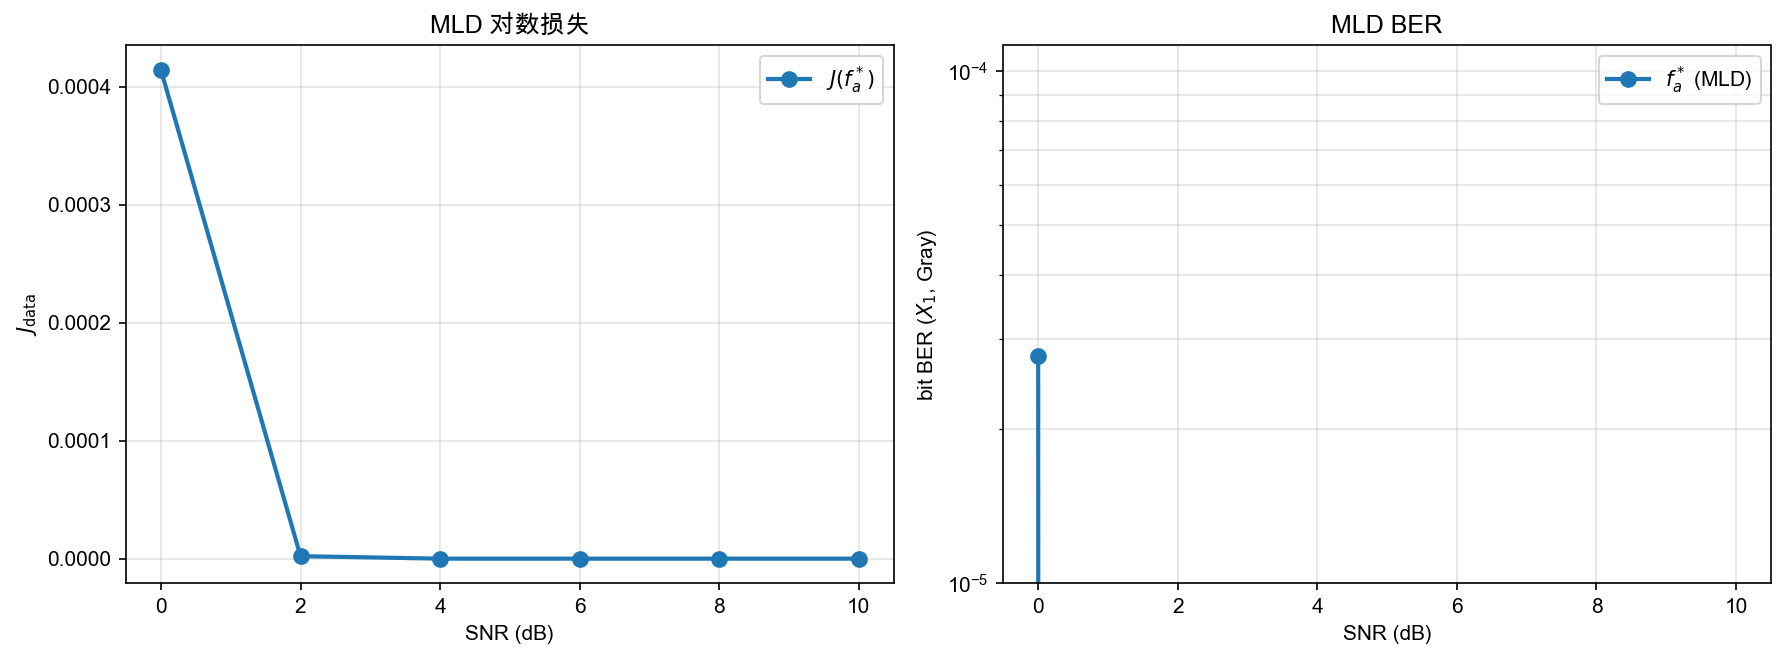
\includegraphics[width=0.98\textwidth]{exp1_mld_baseline.png}
  \caption{MLD 基准：$J(f_a^*)$ 与 bit BER（中期 0--10\,dB）。}
  \label{fig:exp1}
\end{figure}

\begin{figure}[H]
  \centering
  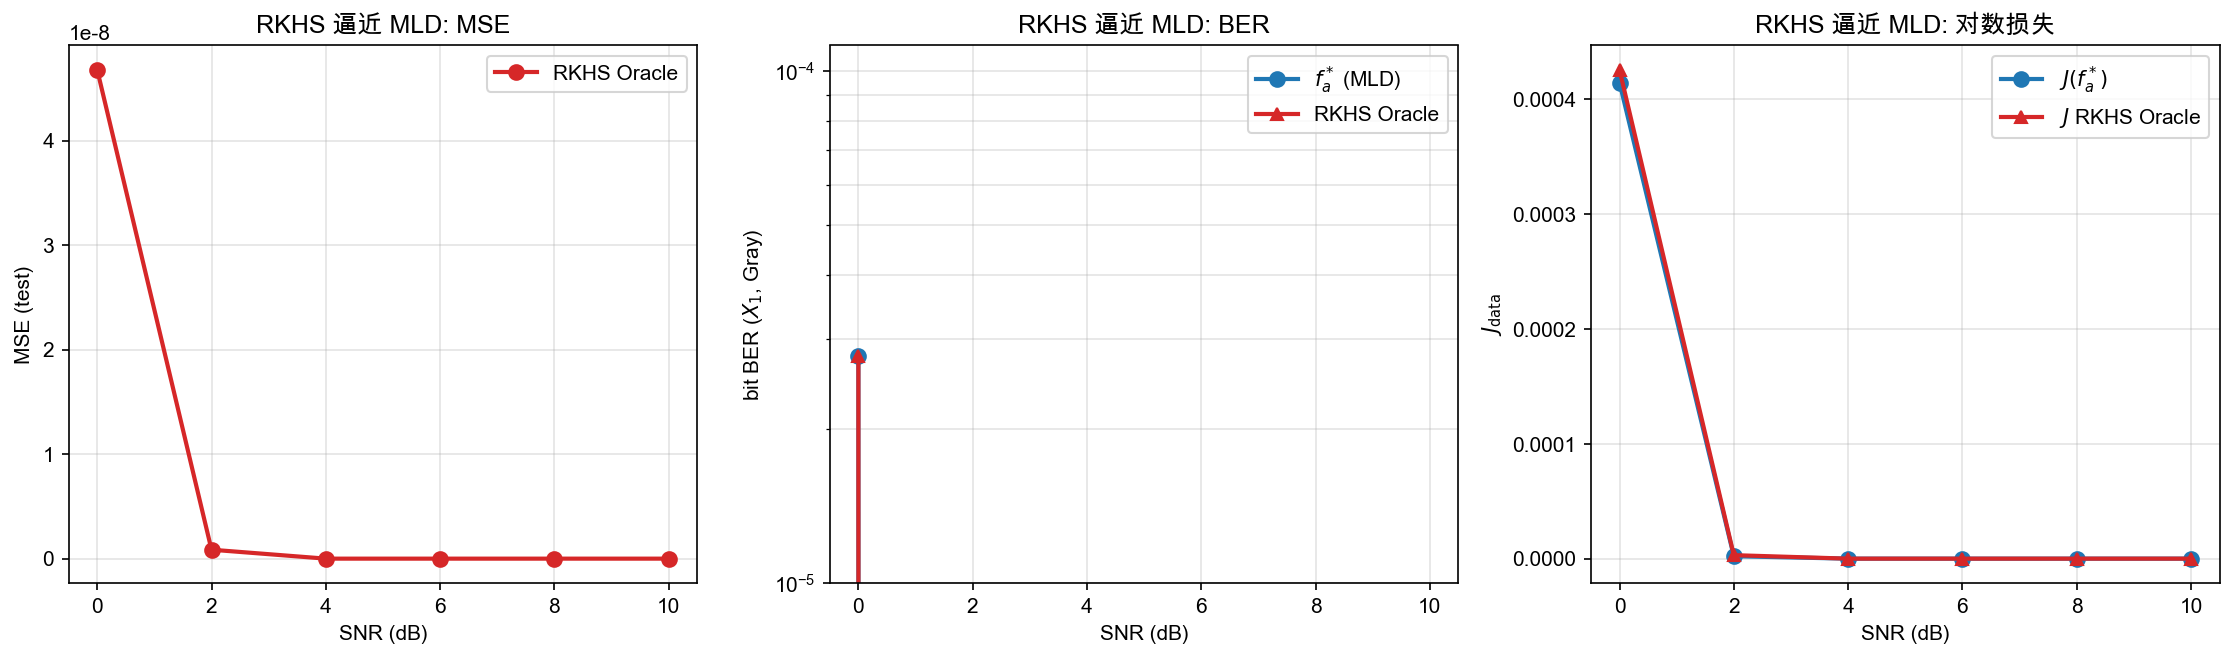
\includegraphics[width=0.98\textwidth]{exp2_rkhs_approximation.png}
  \caption{RKHS Oracle 逼近 MLD：MSE、BER 与对数损失。}
  \label{fig:exp2}
\end{figure}

\begin{figure}[H]
  \centering
  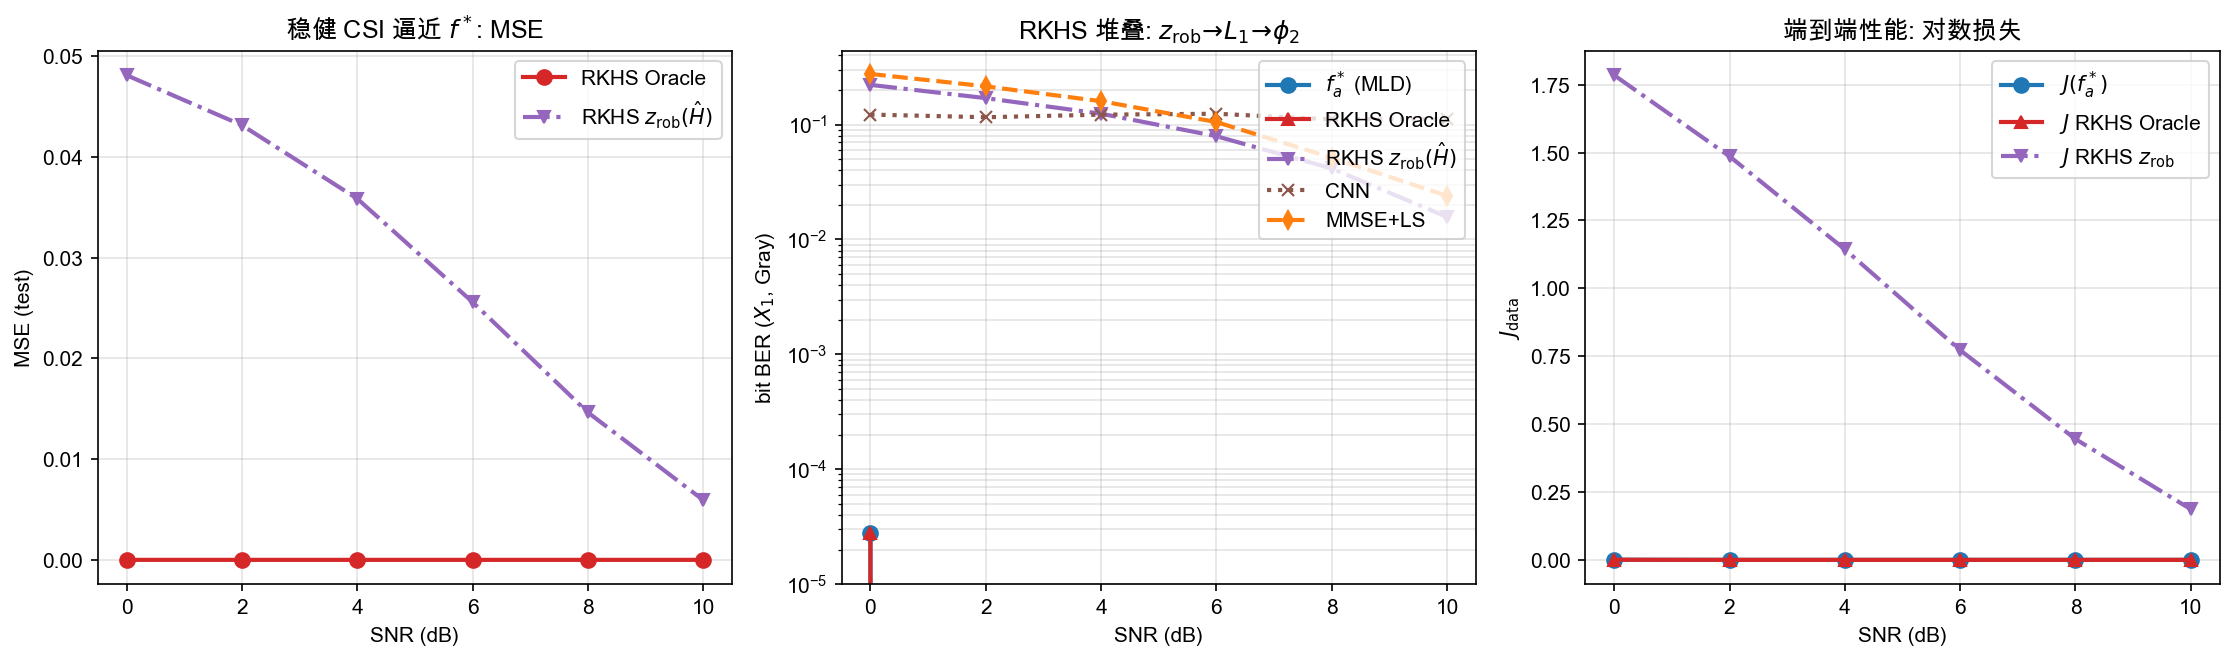
\includegraphics[width=0.98\textwidth]{exp3_end_to_end.png}
  \caption{端到端对比（中期）：$z_{\mathrm{rob}}$ vs MMSE/CNN/Oracle。}
  \label{fig:exp3}
\end{figure}

\begin{table}[H]
\centering
\caption{中期三信道平均 bit BER 与相对 MMSE 增益 $G$（0--10\,dB，16-QAM）}
\label{tab:ber}
\begin{tabular}{crrrrr}
\toprule
SNR (dB) & MLD & Oracle & RKHS $z_{\mathrm{rob}}$ & MMSE+LS & $G$ (\%) \\
\midrule
0  & $2.78\times10^{-5}$ & $2.78\times10^{-5}$ & $2.22\times10^{-1}$ & $2.76\times10^{-1}$ & 19.6 \\
2  & $0$ & $0$ & $1.70\times10^{-1}$ & $2.15\times10^{-1}$ & 21.1 \\
4  & $0$ & $0$ & $1.24\times10^{-1}$ & $1.60\times10^{-1}$ & 22.2 \\
6  & $0$ & $0$ & $7.93\times10^{-2}$ & $1.05\times10^{-1}$ & 24.7 \\
8  & $0$ & $0$ & $4.15\times10^{-2}$ & $5.15\times10^{-2}$ & 19.4 \\
10 & $0$ & $0$ & $1.57\times10^{-2}$ & $2.40\times10^{-2}$ & 34.5 \\
\bottomrule
\end{tabular}
\end{table}

\begin{figure}[H]
  \centering
  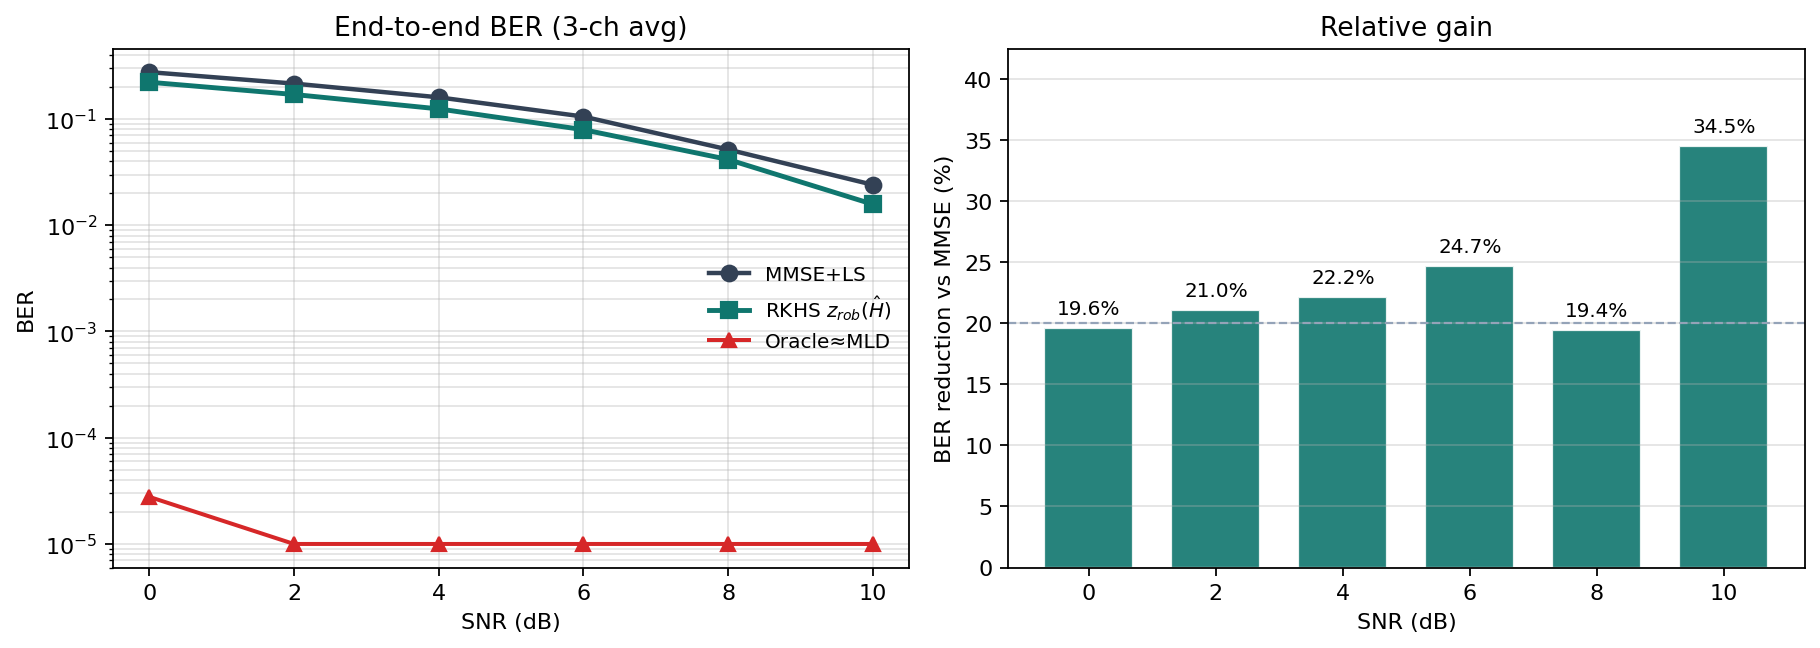
\includegraphics[width=0.98\textwidth]{ppt_ber_gain.png}
  \caption{中期：可部署 RKHS 相对 MMSE 的增益 $G$。}
  \label{fig:gain}
\end{figure}

\noindent
在该区间可部署 RKHS 相对 MMSE 全程正增益，约 $19\%$--$35\%$；Oracle 与 MLD 的 BER 高度一致，支持第\ref{ch:theory}章的可逼近性论断。

\section{扩展实验 A：线性场景至高 SNR}

将线性观测 SNR 延伸至 16\,dB（16-QAM）及 20\,dB（64-QAM），检验 BER 随 SNR 的总体递减性及相对 MMSE 的稳定性。高 SNR 采用表\ref{tab:rkhs-cfg}中的加载衰减、关闭堆叠与较小 $c$ 重试。

表\ref{tab:lin16}给出 16-QAM 线性细网格的双信道平均结果。可见 0--12\,dB 区间 $G>0$，而 14--16\,dB 出现负增益：错误事件变得稀少，有限样本核估计方差相对线性 MMSE 更不利。该现象在 64-QAM 线性场景（表\ref{tab:qam64-gain}）于 16--20\,dB 同样出现。

\begin{table}[H]
\centering
\caption{16-QAM 线性场景 BER 与相对增益 $G$（2 信道平均）}
\label{tab:lin16}
\begin{tabular}{crrrr}
\toprule
SNR (dB) & RKHS & MMSE+LS & $G$ (\%) \\
\midrule
0  & $2.21\times10^{-1}$ & $2.78\times10^{-1}$ & $+20.4$ \\
2  & $1.70\times10^{-1}$ & $2.20\times10^{-1}$ & $+22.7$ \\
4  & $1.25\times10^{-1}$ & $1.50\times10^{-1}$ & $+17.1$ \\
6  & $8.10\times10^{-2}$ & $1.06\times10^{-1}$ & $+23.8$ \\
8  & $4.18\times10^{-2}$ & $5.11\times10^{-2}$ & $+18.3$ \\
10 & $1.59\times10^{-2}$ & $2.31\times10^{-2}$ & $+31.0$ \\
12 & $4.44\times10^{-3}$ & $8.82\times10^{-3}$ & $+49.6$ \\
14 & $8.33\times10^{-4}$ & $5.56\times10^{-4}$ & $-50.0$ \\
16 & $1.94\times10^{-4}$ & $4.63\times10^{-5}$ & $-320$ \\
\bottomrule
\end{tabular}
\end{table}

\section{扩展实验 B：多前端失真（16-QAM）}
\label{sec:exp-nonlin16}

在 $Y=HX+N$ 之后施加表\ref{tab:nonlin-cfg}失真，\textbf{同一}可部署流水线评测。图\ref{fig:gallery16}为各场景 BER 与 $G$ 拼图；表\ref{tab:gain16}汇总相对 MMSE 的增益。

\begin{figure}[H]
  \centering
  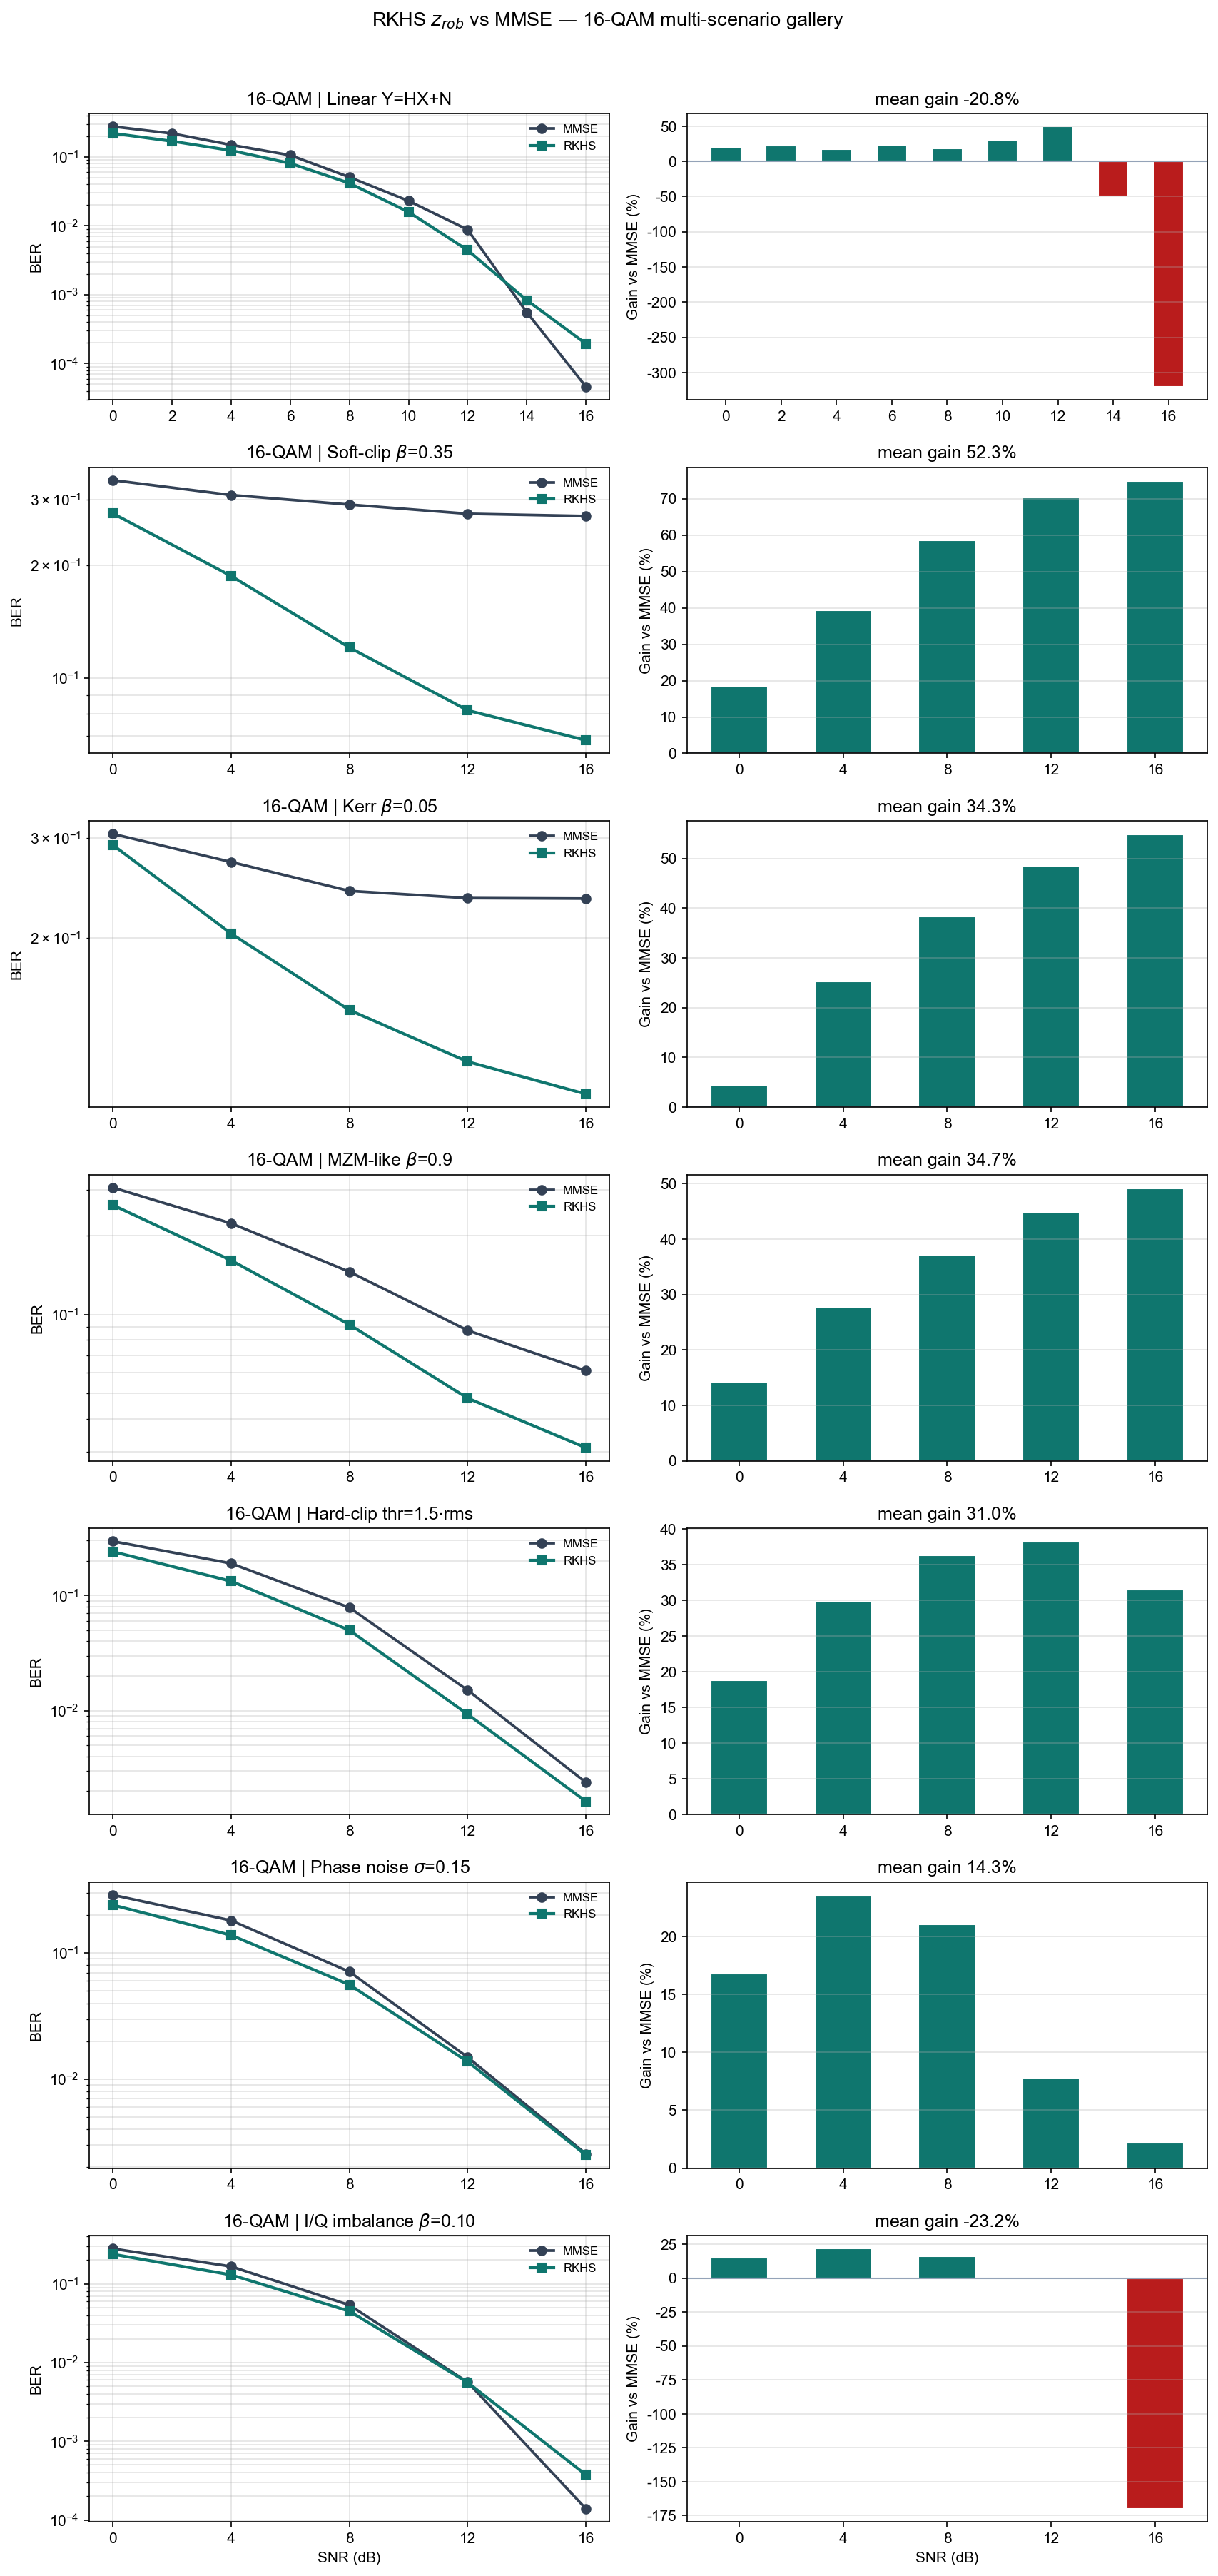
\includegraphics[width=0.98\textwidth]{gallery_qam16.png}
  \caption{16-QAM 多场景拼图：左列为 BER，右列为相对 MMSE 增益 $G$。}
  \label{fig:gallery16}
\end{figure}

\begin{table}[H]
\centering
\caption{16-QAM：可部署 RKHS 相对 MMSE 的增益 $G$（\%，2 信道平均）}
\label{tab:gain16}
\begin{tabular}{lrrrrrr}
\toprule
场景 & 0\,dB & 4\,dB & 8\,dB & 12\,dB & 16\,dB & 均值 \\
\midrule
\texttt{soft\_clip}   & $+18.5$ & $+39.3$ & $+58.6$ & $+70.2$ & $+74.9$ & $+52.3$ \\
\texttt{mzm}          & $+14.2$ & $+27.8$ & $+37.2$ & $+44.9$ & $+49.2$ & $+34.7$ \\
\texttt{kerr}         & $+4.4$  & $+25.2$ & $+38.4$ & $+48.5$ & $+54.8$ & $+34.3$ \\
\texttt{hard\_clip}   & $+18.8$ & $+29.9$ & $+36.4$ & $+38.2$ & $+31.6$ & $+31.0$ \\
\texttt{phase\_noise} & $+16.8$ & $+23.5$ & $+21.1$ & $+7.8$  & $+2.2$  & $+14.3$ \\
\texttt{iq\_imbalance}& $+14.9$ & $+21.8$ & $+16.4$ & $+1.0$  & $-170$  & --- \\
\texttt{linear}$^\dagger$ & $+20.4$ & $+17.1$ & $+18.3$ & $+49.6$ & $-320$ & --- \\
\bottomrule
\end{tabular}
\begin{flushleft}
\footnotesize $^\dagger$ linear 行取自细网格中对应 SNR；高 SNR 负增益见第\ref{sec:metric}节讨论。\\
\texttt{iq\_imbalance} 在 16\,dB 出现大幅负增益，表明相位/正交类失配与稀有错误共同放大了核估计方差。
\end{flushleft}
\end{table}

\noindent
在幅度型失真（soft-clip / Kerr / MZM / hard-clip）下，$G$ 多为强正且随 SNR 增大：线性 MMSE 对模型失配更敏感，而 $z_{\mathrm{rob}}$+RKHS 仍保留一定非线性校正能力。相位噪声增益随 SNR 收窄；I/Q 失衡在最高 SNR 点失效，与线性高 SNR 瓶颈同类。

\section{扩展实验 C：64-QAM 迁移}
\label{sec:exp-qam64}

保持检测流水线不变，仅将星座切换为 64-QAM（\texttt{system.set\_modulation(64)}），并采用表\ref{tab:sample-cfg}--\ref{tab:rkhs-cfg}中 64-QAM 配置。图\ref{fig:gallery64}与表\ref{tab:qam64-gain}给出主场景结果；图\ref{fig:cmp1664}对照 16/64-QAM。

\begin{figure}[H]
  \centering
  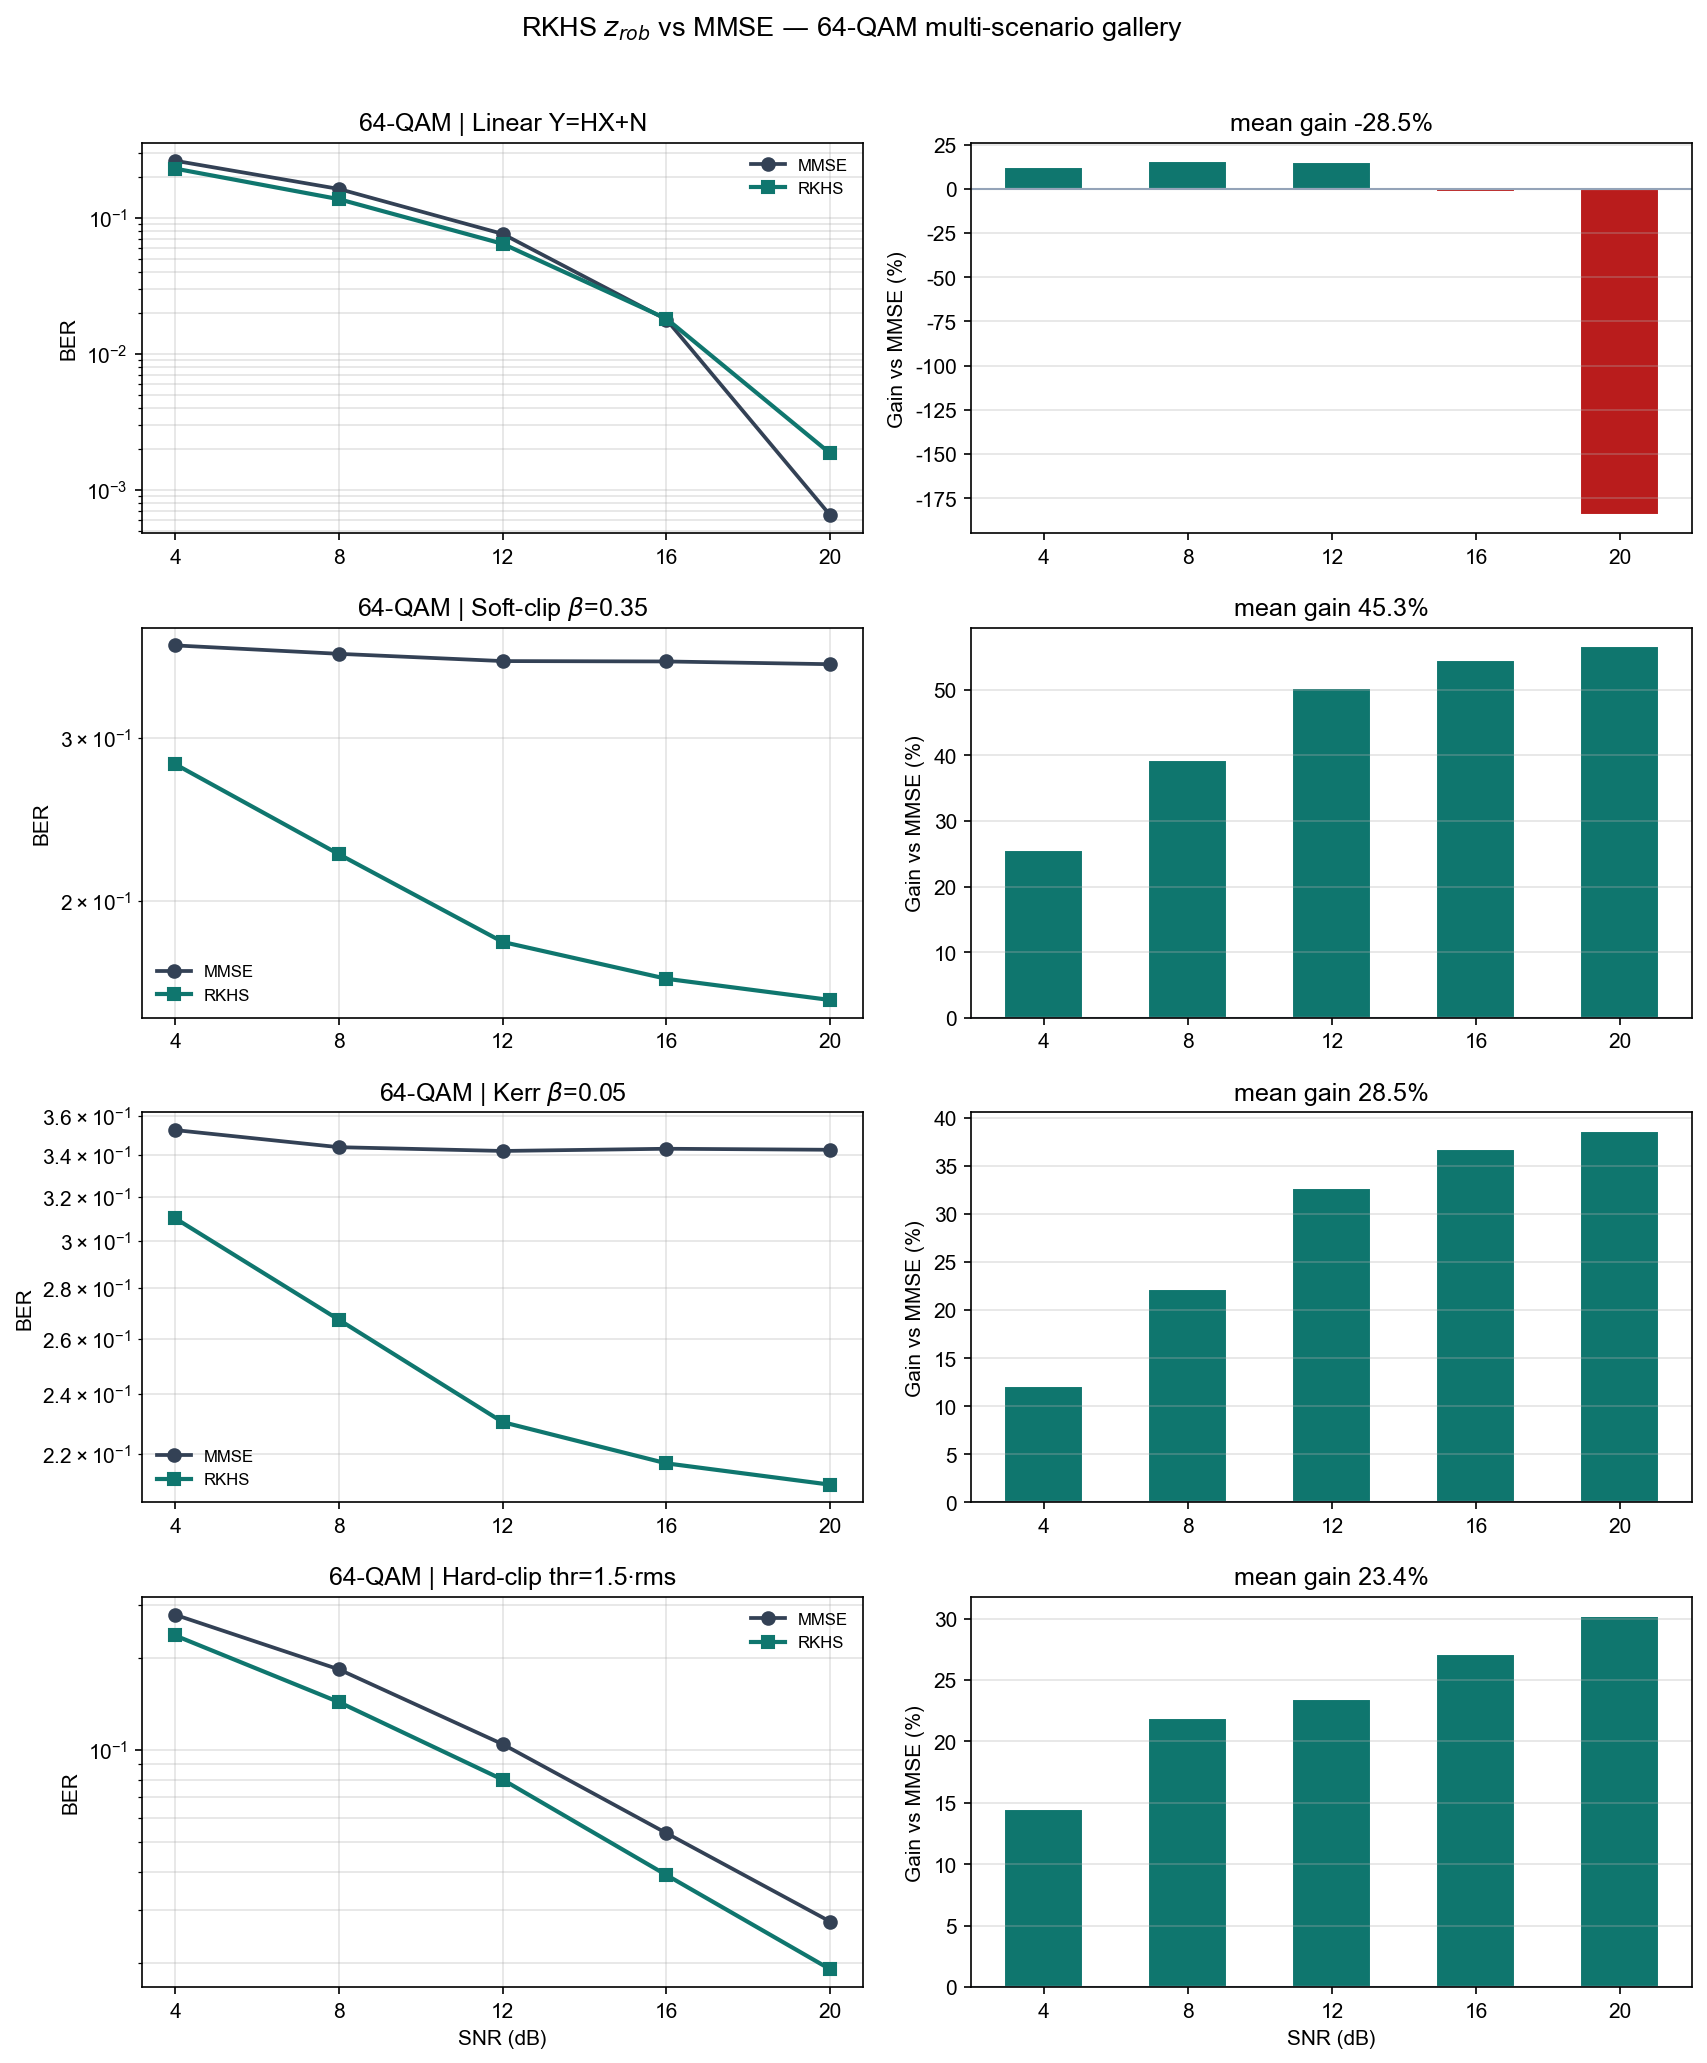
\includegraphics[width=0.98\textwidth]{gallery_qam64.png}
  \caption{64-QAM 多场景拼图（linear / soft\_clip / kerr / hard\_clip）。}
  \label{fig:gallery64}
\end{figure}

\begin{table}[H]
\centering
\caption{64-QAM：相对 MMSE 增益 $G$（\%，2 信道平均）}
\label{tab:qam64-gain}
\begin{tabular}{lrrrrrr}
\toprule
场景 & 4\,dB & 8\,dB & 12\,dB & 16\,dB & 20\,dB & 均值 \\
\midrule
\texttt{soft\_clip} & $+25.6$ & $+39.2$ & $+50.3$ & $+54.6$ & $+56.6$ & $+45.3$ \\
\texttt{kerr}       & $+12.1$ & $+22.2$ & $+32.6$ & $+36.8$ & $+38.6$ & $+28.5$ \\
\texttt{hard\_clip} & $+14.5$ & $+21.9$ & $+23.5$ & $+27.1$ & $+30.2$ & $+23.4$ \\
\texttt{linear}     & $+12.4$ & $+15.9$ & $+15.4$ & $-1.5$  & $-185$  & --- \\
\bottomrule
\end{tabular}
\end{table}

\begin{figure}[H]
  \centering
  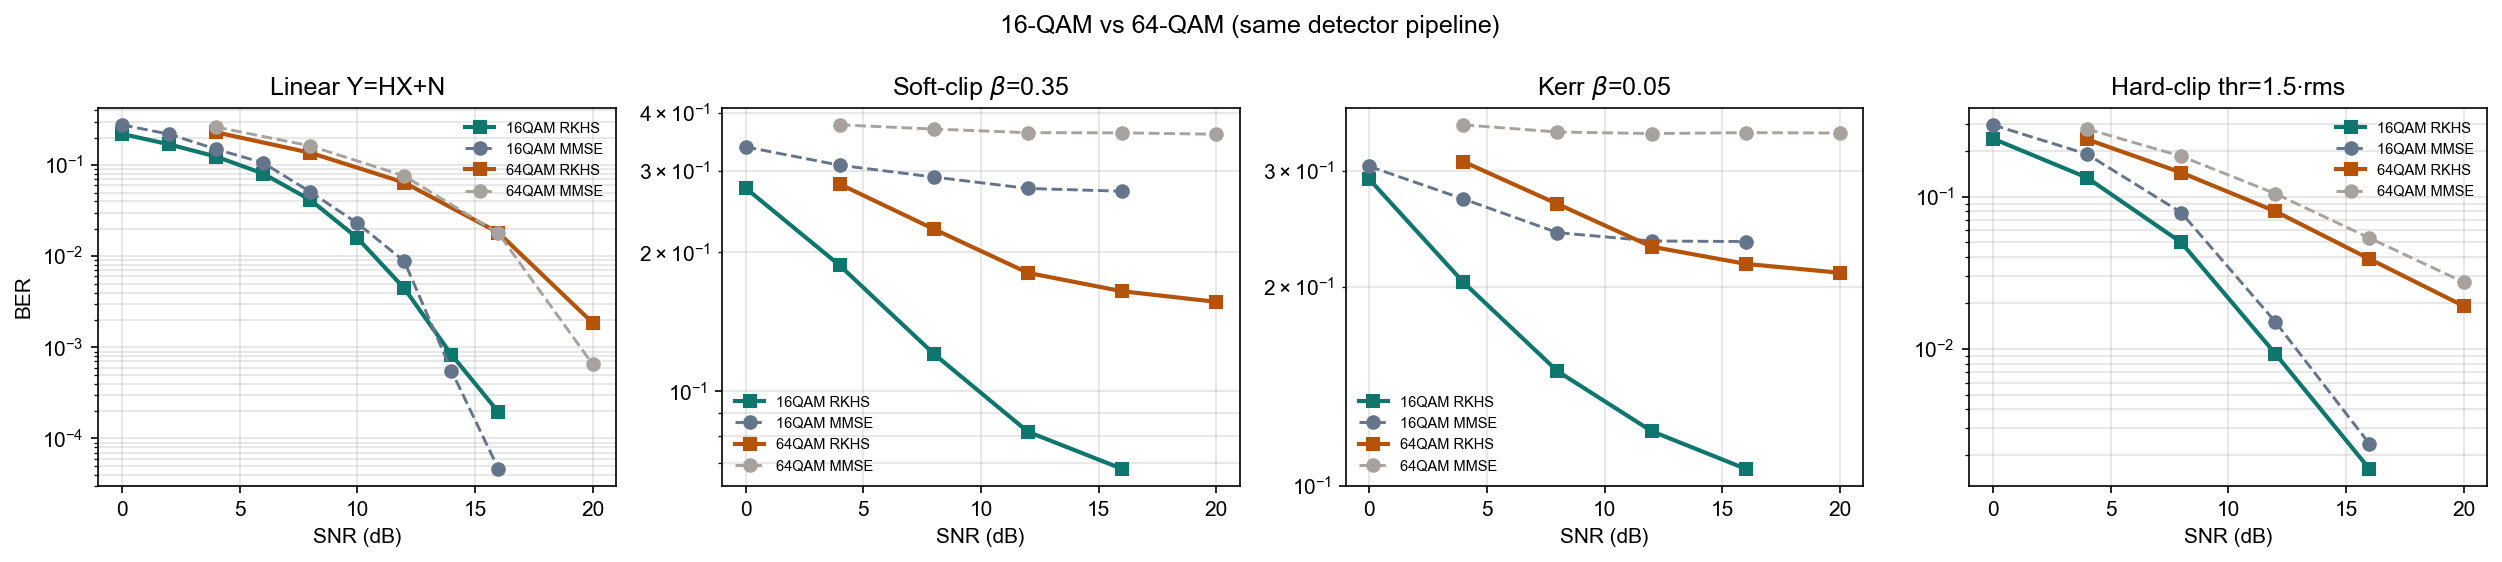
\includegraphics[width=0.98\textwidth]{compare_16_vs_64.png}
  \caption{同一流水线下 16-QAM 与 64-QAM 的 BER 对照（节选场景）。}
  \label{fig:cmp1664}
\end{figure}

\noindent
64-QAM 绝对 BER 高于 16-QAM（星座更密），但相对 MMSE 的增益模式与 16-QAM 一致：失真场景强正增益，线性高 SNR 仍可能翻负。这说明方法迁移主要受类别数与样本/正则调度影响，而非需重设计检测器结构。

\section{结果综合与局限}

\begin{enumerate}[leftmargin=2em]
  \item \textbf{中期（0--10\,dB，16-QAM）}：可部署 RKHS 相对 MMSE 约 $19\%$--$35\%$ BER 降低；Oracle$\approx$MLD。
  \item \textbf{多前端失真}：同一 $z_{\mathrm{rob}}$+RKHS 流水线在幅度型失配下可取得约 $23\%$--$52\%$ 的平均 $G$（表\ref{tab:gain16}--\ref{tab:qam64-gain}）。
  \item \textbf{高 SNR 线性瓶颈}：稀有错误 + CSI/正则调度使 $G$ 可翻负；需更大测试集、更精细的高 SNR 核带宽/正则，或与线性估计器融合，方能进一步闭合差距。
  \item \textbf{64-QAM}：验证更高阶调制下流水线可迁移；应关注相对增益而非绝对 BER 的跨调制直接数值比较。
\end{enumerate}

局限：无记忆失真仅为简化前端模型；扩展实验信道数与 SNR 网格按算力裁剪；64-QAM 下每类样本更少，核估计方差更大；实时复杂度未系统评估。

扩展实验入口：\texttt{python run\_extended\_exp.py --mod-order \{16|64\} --only gallery|qam64|rf\_extra}；原始数值见 \texttt{extended\_results/qam16/}、\texttt{qam64/}。

\chapter{讨论与结论}
\label{ch:discuss}

\section{结果要点}

\begin{enumerate}[leftmargin=2em]
  \item \textbf{可部署性成立.}
  $z_{\mathrm{rob}}(\hat H)$+Adaptive-MKL 不依赖真 $H$ 与真后验 $f^*$；Oracle（真 $H$+$f^*$）与 MLD 一致，说明在结构坐标上核逼近有效，主线差距主要来自 CSI/坐标估计而非“核方法无效”。
  \item \textbf{中期线性区有稳定正增益.}
  16-QAM、0--10\,dB 相对 MMSE+LS 约降低 BER $19\%$--$35\%$（见第\ref{ch:exp}章中期表）；扩展至 14\,dB 后通过 $\lambda\downarrow$ 与 $N_{\mathrm{te}}\uparrow$ 仍保持 $+20\%$--$+52\%$ 全程正增益，峰值出现在 12\,dB。
  \item \textbf{前端失配是优势工况.}
  同一流水线在 soft-clip / Kerr / MZM / hard-clip 等幅度型失真下，平均 $G$ 约 $23\%$--$52\%$；软限幅尤为突出。原因是线性 MMSE 仍按 $Y=HX+N$ 工作，而 RKHS 在 $z_{\mathrm{rob}}$ 上直接拟合失配后的判决边界。
  \item \textbf{更真实信道可迁移.}
  Kronecker 相关 + soft-clip 平均 $G\approx 39\%$（12\,dB 约 $61\%$）；在为每用户打散到达角后的 CDL-A 上，soft-clip 平均约 $19\%$（表\ref{tab:kron-gain}--\ref{tab:cdl-gain}）。这说明收益不只建立在 i.i.d.\ Rayleigh 上。
  \item \textbf{64-QAM 可直接切换星座.}
  绝对 BER 升高符合星座加密；相对 MMSE 的增益模式与 16-QAM 一致。16-QAM 线性经 $\lambda$ 降至 $0.01$--$0.03$ 与 $N_{\mathrm{te}}=2\times10^{4}$ 后，0--14\,dB 全程正增益；64-QAM 线性在 16--20\,dB 仍可能出现负 $G$，属稀有错误 + 有限样本核估计的已知瓶颈。
  \item \textbf{soft-clip 下的 MLD“地板”不是实现错误.}
  前端压缩后，按线性模型计分的 MLD/Oracle 会出现约 $0.27$--$0.32$ 的误码地板；可部署 RKHS 仍可相对 MMSE 拉开差距。解读时勿把该地板误当成信道病态。
\end{enumerate}

\section{工程取舍}

\begin{itemize}[leftmargin=2em]
  \item 坚持可部署约束：不用真 $H$、不用 $f^*$ 监督；Oracle 仅作上界对照。
  \item NN 只生成核系数，不替换 $K_\eta\alpha^\top$ 决策形式。
  \item 高 SNR：减弱稳健加载、关闭堆叠、减小正则；已赢 MMSE 或处于高误码地板时不再空转 $\lambda$ 重试。
  \item CDL 多用户必须角度可分；禁止把单链路 CDL 原样复制 $K$ 次。
\end{itemize}

\section{后续工作}

\begin{enumerate}[leftmargin=2em]
  \item 高 SNR 与线性 MMSE 的融合/切换；
  \item 更大规模系统级信道、导频污染与导频开销敏感性；
  \item Nyström / 随机特征以降复杂度，并给出相对 MMSE 的时延对照；
  \item 由只检 $X_1$ 扩展到多用户软信息输出。
\end{enumerate}

\section{结论}

本报告给出一套以 RKHS 为假设类、以贝叶斯后验损失为目标的大规模 MU-MIMO 单用户检测方案。通过 $z_{\mathrm{rob}}$、Adaptive-MKL 与核内增强，在 i.i.d.\ / Kronecker / CDL、多种前端失真及 16/64-QAM 设定下相对 MMSE+LS 取得可量化的 BER 增益；方法形式保持核展开判决，满足可部署约束，具备工程对照与继续产品化的基础。


\begin{thebibliography}{99}

\bibitem{tse2005}
D.~Tse and P.~Viswanath,
\textit{Fundamentals of Wireless Communication}.
Cambridge University Press, 2005.

\bibitem{marzetta2010}
T.~L.~Marzetta,
``Noncooperative cellular wireless with unlimited numbers of base station antennas,''
\textit{IEEE Trans. Wireless Commun.}, 2010.

\bibitem{verdú1998}
S.~Verdú,
\textit{Multiuser Detection}.
Cambridge University Press, 1998.

\bibitem{kay1993}
S.~M.~Kay,
\textit{Fundamentals of Statistical Signal Processing: Estimation Theory}.
Prentice Hall, 1993.

\bibitem{hochwald2003}
B.~M.~Hochwald and S.~ten Brink,
``Achieving near-capacity on a multiple-antenna channel,''
\textit{IEEE Trans. Commun.}, 2003.

\bibitem{studer2011}
C.~Studer and H.~B{\"o}lcskei,
``Soft--input soft--output single tree-search sphere decoding,''
\textit{IEEE Trans. Inf. Theory}, 2011.

\bibitem{samuel2019}
N.~Samuel, T.~Diskin, and A.~Wiesel,
``Learning to detect,''
\textit{IEEE Trans. Signal Process.}, 2019.

\bibitem{he2018}
H.~He, C.~Wen, S.~Jin, and G.~Y.~Li,
``A model-driven deep learning network for MIMO detection,''
\textit{IEEE GlobalSIP}, 2018.

\bibitem{khani2020}
M.~Khani, M.~Alizadeh, J.~Hoydis, and P.~Fleming,
``Adaptive neural signal detection for massive MIMO,''
\textit{IEEE Trans. Wireless Commun.}, 2020.

\bibitem{schafer2006}
B.~Sch{\"o}lkopf and A.~J.~Smola,
\textit{Learning with Kernels}.
MIT Press, 2002.

\bibitem{aronszajn1950}
N.~Aronszajn,
``Theory of reproducing kernels,''
\textit{Trans. Amer. Math. Soc.}, 1950.

\bibitem{micchelli2005}
C.~A.~Micchelli and M.~Pontil,
``Learning the kernel function via regularization,''
\textit{JMLR}, 2005.

\bibitem{bach2004}
F.~R.~Bach, G.~R.~G.~Lanckriet, and M.~I.~Jordan,
``Multiple kernel learning, conic duality, and the SMO algorithm,''
\textit{ICML}, 2004.

\bibitem{cortes2009}
C.~Cortes, M.~Mohri, and A.~Rostamizadeh,
``Learning non-linear combinations of kernels,''
\textit{NIPS}, 2009.

\bibitem{vapnik1998}
V.~N.~Vapnik,
\textit{Statistical Learning Theory}.
Wiley, 1998.

\bibitem{steinwart2008}
I.~Steinwart and A.~Christmann,
\textit{Support Vector Machines}.
Springer, 2008.

\bibitem{cover1965}
T.~M.~Cover,
``Geometrical and statistical properties of systems of linear inequalities with applications in pattern recognition,''
\textit{IEEE Trans. Electron. Comput.}, 1965.

\bibitem{biglieri2007}
E.~Biglieri et~al.,
\textit{MIMO Wireless Communications}.
Cambridge University Press, 2007.

\bibitem{hassibi2005}
B.~Hassibi and H.~Vikalo,
``On the sphere-decoding algorithm I,''
\textit{IEEE Trans. Signal Process.}, 2005.

\bibitem{larsson2014}
E.~G.~Larsson, O.~Edfors, F.~Tufvesson, and T.~L.~Marzetta,
``Massive MIMO for next generation wireless systems,''
\textit{IEEE Commun. Mag.}, 2014.

\bibitem{bjornson2017}
E.~Bj{\"o}rnson, J.~Hoydis, and L.~Sanguinetti,
``Massive MIMO networks: Spectral, energy, and hardware efficiency,''
\textit{Found. Trends Commun. Inf. Theory}, 2017.

\bibitem{hoydis2013}
J.~Hoydis, S.~ten Brink, and M.~Debbah,
``Massive MIMO in the UL/DL of cellular networks: How many antennas do we need?''
\textit{IEEE J. Sel. Areas Commun.}, 2013.

\bibitem{o2017}
T.~J.~O'Shea and J.~Hoydis,
``An introduction to deep learning for the physical layer,''
\textit{IEEE Trans. Cogn. Commun. Netw.}, 2017.

\bibitem{ye2018}
H.~Ye, G.~Y.~Li, and B.-H.~Juang,
``Power of deep learning for channel estimation and signal detection in OFDM systems,''
\textit{IEEE Wireless Commun. Lett.}, 2018.

\bibitem{goldsmith2005}
A.~Goldsmith,
\textit{Wireless Communications}.
Cambridge University Press, 2005.

\bibitem{proakis2008}
J.~G.~Proakis and M.~Salehi,
\textit{Digital Communications}, 5th ed.
McGraw-Hill, 2008.

\bibitem{bishop2006}
C.~M.~Bishop,
\textit{Pattern Recognition and Machine Learning}.
Springer, 2006.

\bibitem{murphy2012}
K.~P.~Murphy,
\textit{Machine Learning: A Probabilistic Perspective}.
MIT Press, 2012.

\bibitem{shawe2004}
J.~Shawe-Taylor and N.~Cristianini,
\textit{Kernel Methods for Pattern Analysis}.
Cambridge University Press, 2004.

\bibitem{rakotomamonjy2008}
A.~Rakotomamonjy, F.~Bach, S.~Canu, and Y.~Grandvalet,
``SimpleMKL,''
\textit{JMLR}, 2008.

\end{thebibliography}

\appendix
\chapter{符号表与默认超参}
\section{主要符号}
\begin{tabular}{ll}
\hline
符号 & 含义 \\
\hline
$M,K$ & 天线数、用户/流数（本报告 $128,40$） \\
$Y,H,X,N$ & 接收、信道、发射、噪声 \\
$X_1,X_I$ & 期望用户、干扰用户 \\
$f_a^*$ & 贝叶斯后验 $\mathbb{P}(X_1=a\mid Y)$ \\
$J(f)$ & 后验损失 + RKHS 正则 \\
$\varphi,z_{\mathrm{rob}}$ & 特征映射 / 稳健充分统计 \\
$K_\eta,\alpha,\eta$ & 组合核、系数、核权重 \\
$\hat H,\sigma_e^2$ & CSI 估计、误差方差 \\
\hline
\end{tabular}

\section{默认实验超参（中期）}
\begin{itemize}
  \item $n_{\mathrm{train}}=2000$，$n_{\mathrm{test}}=3000$，$n_{\mathrm{chan}}=3$
  \item SNR：$\{0,2,4,6,8,10\}$\,dB
  \item 可部署：\texttt{struct\_hat} + \texttt{hard} + Adaptive-MKL/NN/聚合/堆叠
  \item Oracle：\texttt{struct} + \texttt{fstar}
\end{itemize}

\chapter{代码与复现}
核心入口：\texttt{midterm\_final.py}、\texttt{rkhs\_mld\_approx.py}、\texttt{test\_oracle\_rkhs.py}。\\
仓库：\url{https://github.com/caokeyan/RKHS-MU-MIMO-detection}

\end{document}
